\documentclass[twoside]{protokoll}
\usepackage{graphicx}
\usepackage{tabularx} % for better table formatting
\usepackage{booktabs} % for better table formatting
\usepackage{float} 
\praktikum{I}
\usepackage{subfig}
\usepackage{amsmath}

\versuchsgebiet{(Akustik)}


\teilnehmer{Maximilian Carlos Menke, 434170}
\teilnehmer{Andrea Roth, 428396}
\gruppe{A3}

\begin{document}

\begin{versuchsziele}
\end{versuchsziele}

\section{1E1 Ladekurven eines Kondensators}


\begin{versuchsziele}
Ziel des Versuchs ist die Kapazität eines Kondensators durch lade und entladevorgang
zu bestimmen. 
Dieser wird durch eine Schaltung mit Wiederstand und Schalter ermöglicht.
Hierfür werden verschiedene Methoden verwendet. Mit dem Multimeter werden Kapazität
und Wiederstand bestimmt.
Mit dem Oszilloskop wird über die Zeitkonstante die Kapazität bestimmt. Mit Sensor CASSY 2 zunächst der Wiederstand und dann die Kapazit. 
Diese Ergebnisse sollen dann untereinander verglichen werden.

\end{versuchsziele}


\begin{aufgabe}{Grundlagen}
  Knappe Beschreibung der theoretischen Grundlagen, Angabe der
  benötigten Formel(n), ohne Herleitung. Definition der verwendeten
  Formelzeichen. \\


    Ziel des Versuchs ist es, die Kapazität eines Kondensators zu bestimmen.\\
    Dies können wir messen, da die Spannungsverläufe von Kondensator und Wiederstand mit der Kapazität und dem Wiederstand zusammenhängen.
    Allgemein gilt für einen Kondensator, der aufgeladen wird und mit einem Wiederstand in Reihe geschaltet wurde:
    \begin{equation}
        U_0 - U_C = U_R = I(t) R
        = C\frac{dQ}{dt} R
    \end{equation}
    Diese DGL lässt sich mit Hilfe der seperation der Variablen lösen.
    \begin{equation}
        U_C(t) = U_0 (1 - e^{-\frac{t}{RC}}) = U_0 (1 + e^{\frac{-t}{\tau}})
    \end{equation}
    Für den Strom am Wiederstand ergibt sich damit:
    \begin{equation}
        I(t) = \frac{dQ}{dt} = C * dU_0 = \frac{U_0}{R} * e^{-\frac{t}{RC}} = I_0 * e^{-\frac{t}{\tau}}
    \end{equation}
    Für den Endladevorgan ergibt sich eine änliche DGL:
    \begin{equation}
        U_C(t) = - R I(t)
        = - R C \frac{dU_C}{dt}
    \end{equation}
    Wenn an diese lößt, erhält man:
    \begin{equation}
        \Rightarrow U_C(t) = U_0 (e^{-\frac{t}{RC}})
    \end{equation}
    Für den Strom am Wiederstand kann man jetzt auch leicht mithilfe der Spannung am Kondensator berechnen:
    \begin{equation}
        I(t) = \frac{dQ}{dt} = C dU_0 = \frac{U_0}{R} e^{-\frac{t}{RC}} = I_0 e^{-\frac{t}{\tau}}
    \end{equation}
    Das bedeutet, das wenn man die Konstante $\tau$ bestimmt, z.B 2 Zeit Spannungs Wertepaare bestimmt, da man mit $C = \tau R$ die Kapazität berechnen kann.


\end{aufgabe}

\begin{aufgabe}{Vorversuch: Charakterisierung der verwendeten Bauteile}
  Charakterisieren Sie die verwendeten Bauteile mit Digitalvoltmeter
  und Messbrücke.
  
\subsection{Messung mit Multimeter}
  
  Bevor wir mit dem Versuch angefangen haben, haben wir mit dem Multimeter zunächst die Bauteile charakterisiert, also Wiederstand und Kondensator vermessen.  \\
  
  \textbf{Verwendete Geräte}
  \begin{itemize}
  \item Mulltimeter
  \item Rastersteckplatte DIN A4
  \item 10 $\mu$F Kondensator
  \item 1 k$\Omega$ Wiederstand
  \item Kabel rot/blau
  
  \end{itemize}
  
  Hierfür haben wir den Wiederstand in Reihe mit dem Multimeter gesteckt.
  Den selben Aufbau haben wir für den Kondensator verwendet.
  Der Skizze unten können Sie den Schaltplan für die Messungen entnehmen.
  
  \begin{figure}[H]
      \centering
      \subfloat[Schaltplan messen von R]{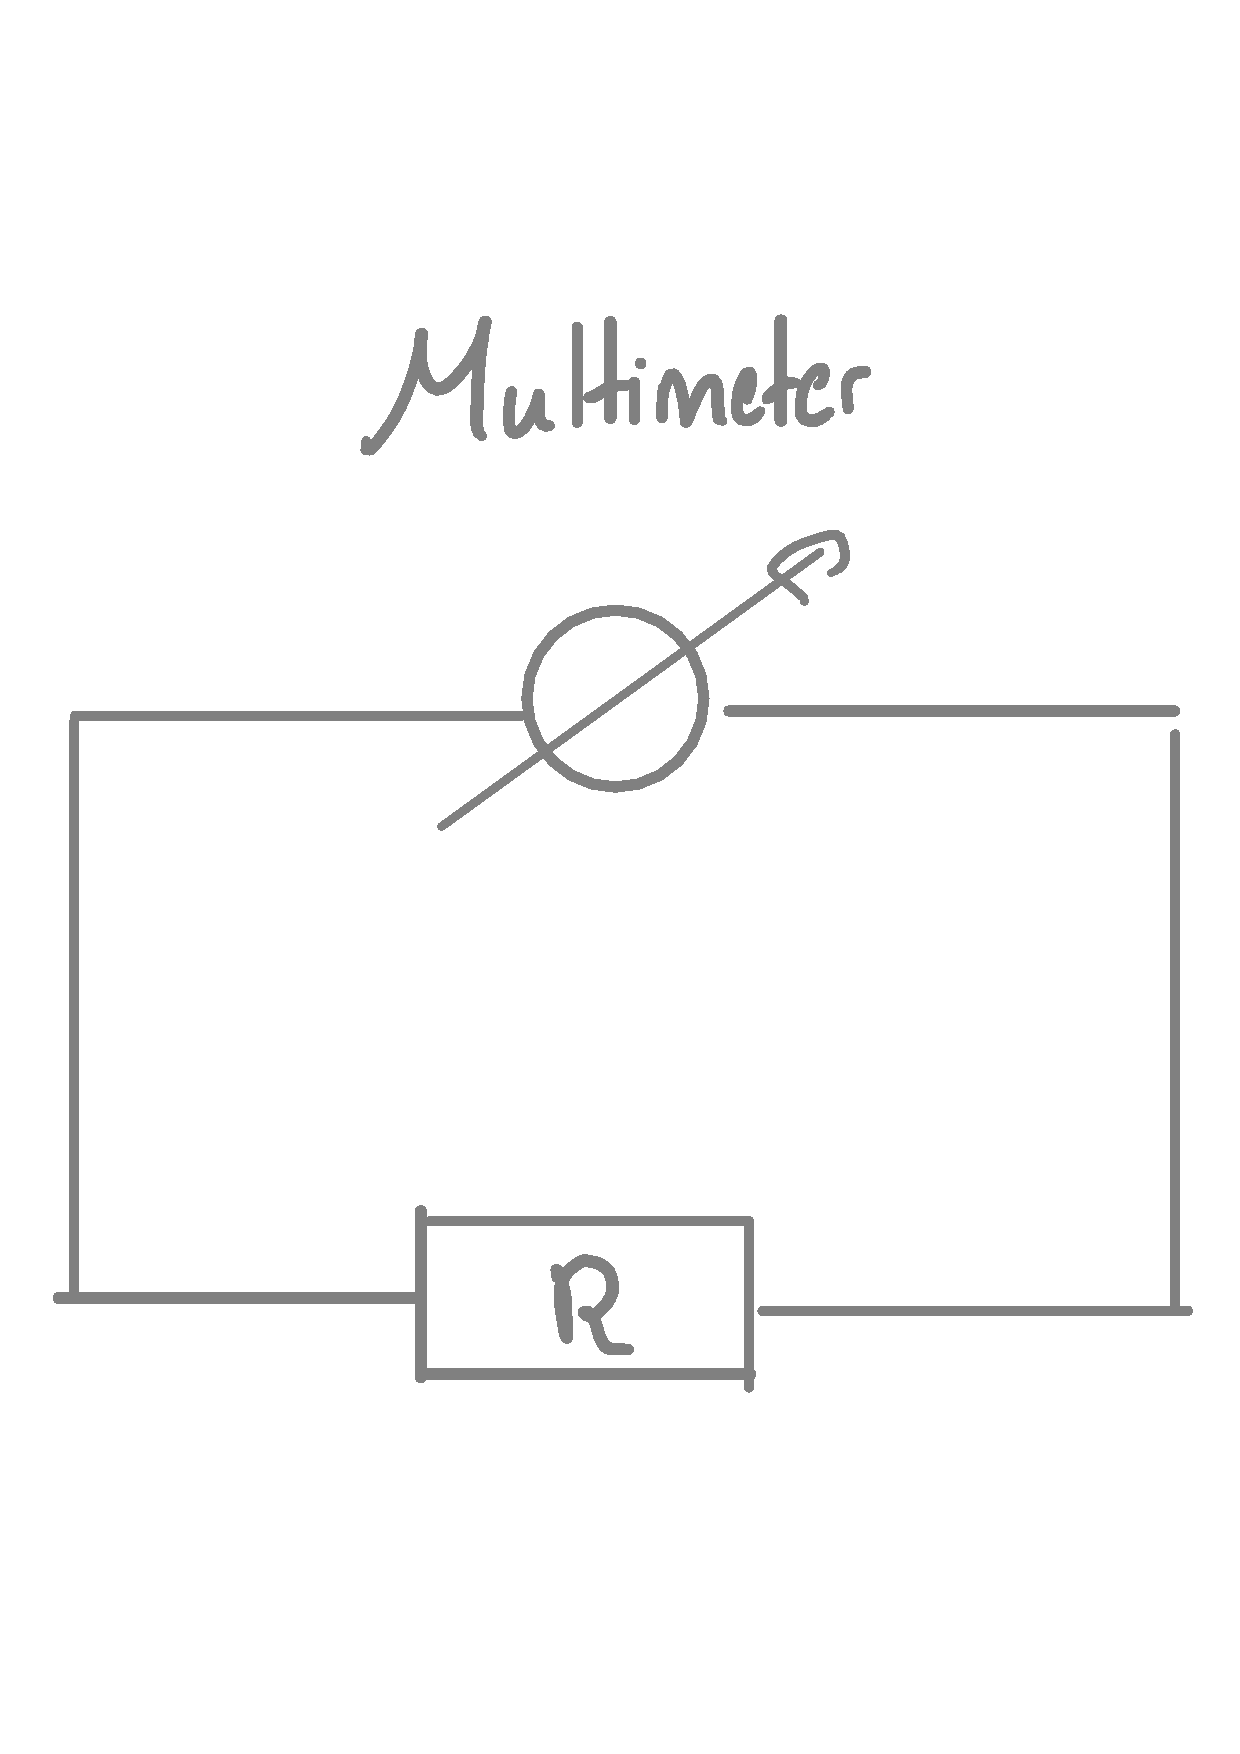
\includegraphics[width=0.5\textwidth]{Schaltung_R_Multimeter.pdf}\label{fig:f1}}
      \hfill
      \subfloat[Schaltplan messen von C]{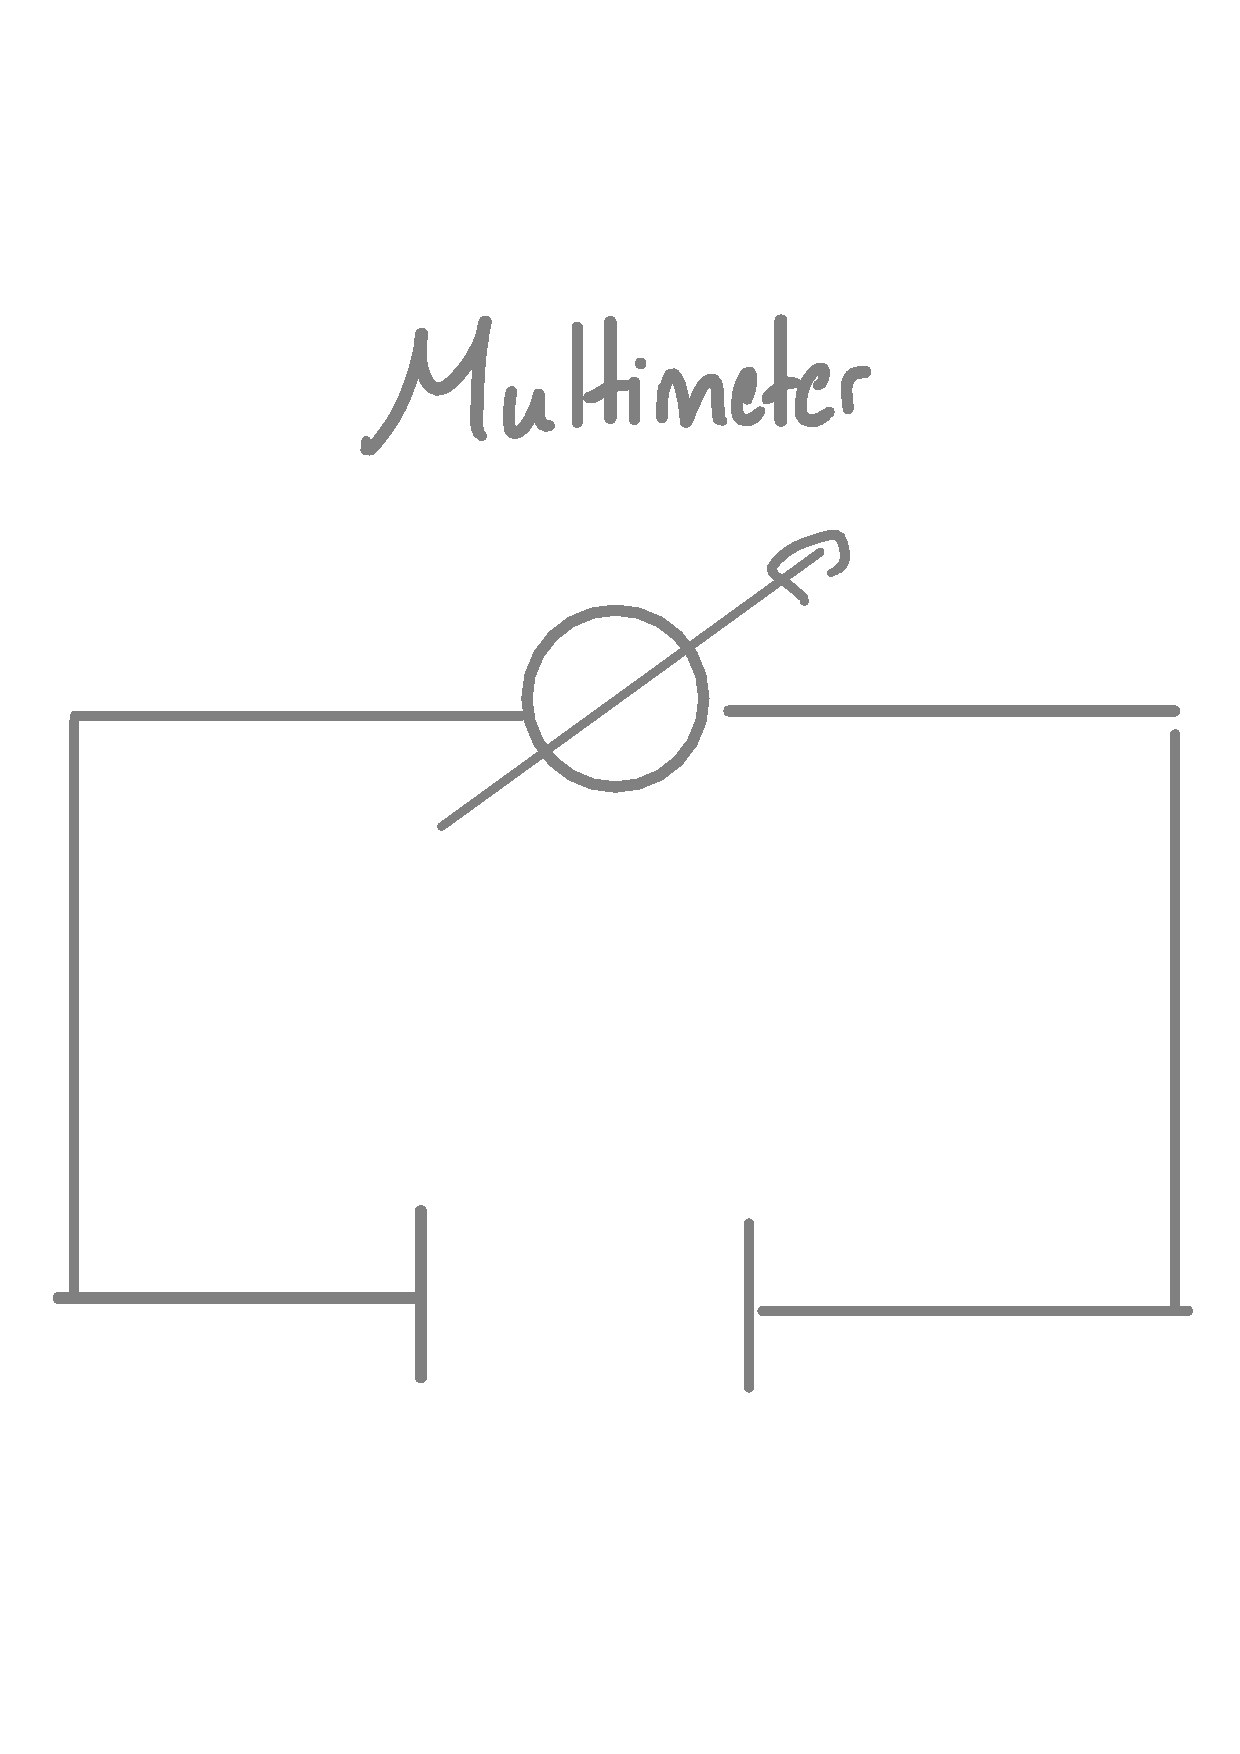
\includegraphics[width=0.5\textwidth]{Schaltung_C_Multimeter.pdf}\label{fig:f2}}
      \caption{Schaltplan für Messungen mit dem Multimeter}
  \end{figure}

Dabei haben wir zur Messung des Wiederstands eines der Kabel an die Masse des Multimeters angeschlossen, und das andere Kabel an die Spannungsbuxe des Multimeters. Da wir wussten, dass wir ein Wiederstand im Bereich 1k$\Omega$ erwarten, haben wir den Drehregler auf 2 k$\Omega$ gestellt.\\ 

Das selbe Vorgehen haben wir beim Messen des Kondensators gewählt, wobei wir hier das zweite Kabel in die Buxe für mA gesteckt, und den Drehregler auf 20 $\mu$F geregelt haben. \\

Die Daten für die Unsicherheiten stammen aus der Bednungsanleitung des Multimeters.\\
\begin{table}[H]
        \centering
        \begin{tabularx}{0.8\textwidth}{X c c} % adjust width as needed
            \toprule
            \textbf{Bauteil} & \textbf{Messung} & \textbf{Fehler} \\
            \midrule
            Wiederstand & 0.991 k$\Omega$ & $\pm$ 0.8\% \\
            Kondensator & 10.36 $\mu$F & $\pm$ 2.5\%  \\
            \bottomrule
        \end{tabularx}
        \caption{Ergebnisse der Messung mit dem Multimeter}
        \label{tab:mytable}
    \end{table}
\end{aufgabe}

\begin{aufgabe}{Vorversuch: Bestimmung des Ohmschen Widerstands}
  Beschreiben Sie den Versuchsaufbau unter Verwendung eines
  Schaltbildes. Beschreiben Sie die Versuchsdurchführung unter Angabe
  der relevanten Messwerterfassungseinstellungen. Zeigen Sie
  exemplarisch die Häufigkeitsverteilungen für Spannung $U$ und Strom
  $I$ an einem Messpunkt und beschreiben Sie, wie Sie die
  statistischen Fehler für $U$ und $I$ bestimmen. Tragen Sie die
  Spannung $U$ gegen den Strom $I$ auf und bestimmen Sie aus der
  Steigung den Widerstand $R$ und seine statistische
  Messunsicherheit. Ermitteln Sie den systematischen Fehler mit der
  Verschiebemethode.\\
  
  \subsection{Aufbau Wiederstandsbestimmung mit CASSY}
  
  Für die Bestimmung des Wiederstands mit dem Sensor CASSY haben wir folgende Geräte verwendet:\\
  
  \textbf{Verwendete Geräte}
  
  \begin{itemize}
  
  \item Sensor CASSY 2
  \item 1 k$\Omega$ Wiederstand
  \item Rastersteckplatte DIN A4
  \item Brückenstecker
  \item Kabel rot/blau
  \end{itemize}
  
Zum Aufbau des Experiments wird der zu messende Wiederstand auf die Steckplatte gesteckt. 
In diesem Versuch soll sowohl Spannung als auch Strom am Wiederstand gemessen werden. Das Schaltbild für diese Messung können sie in der folgenden Skizze sehen. \\

  \begin{figure}[H]
  \centering
  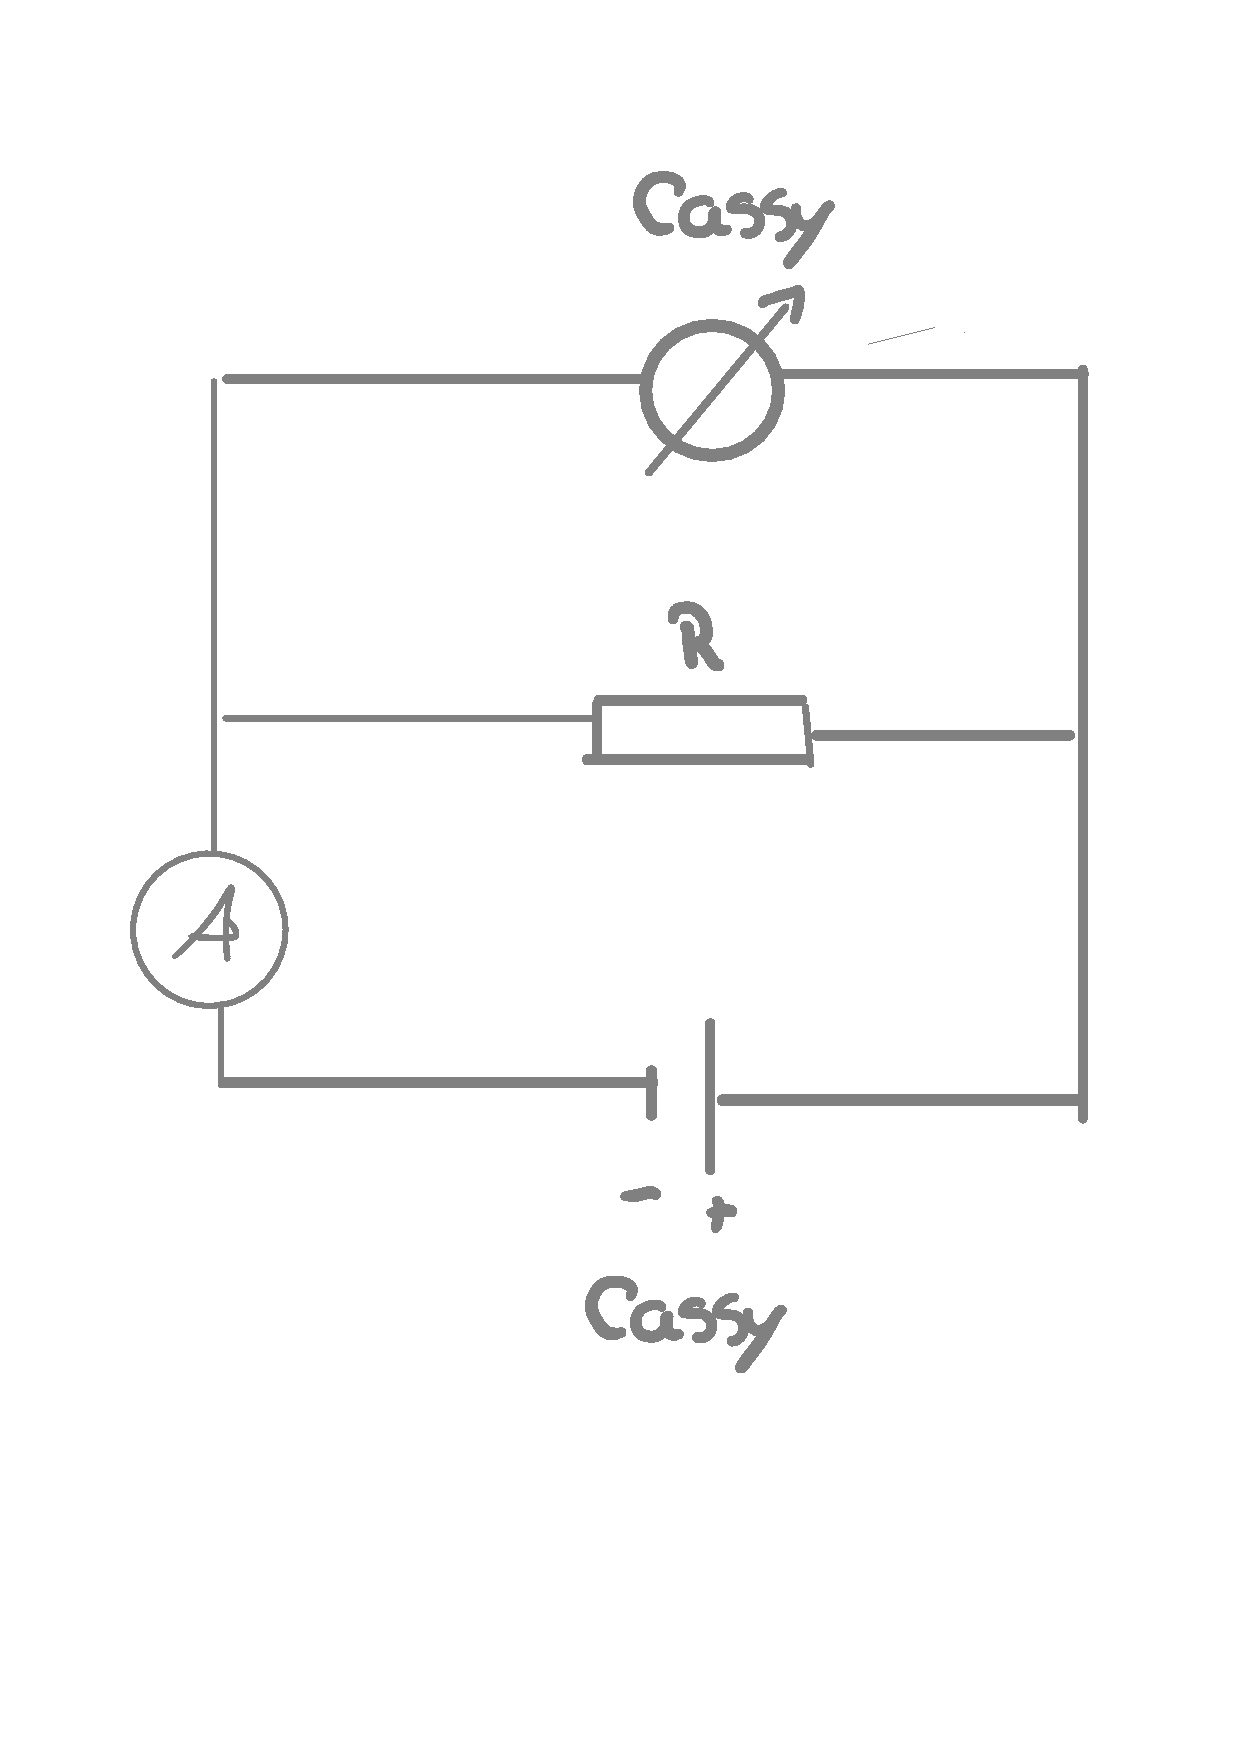
\includegraphics[width=0.7\textwidth]{Schaltung_R_Cassy.pdf}
  \caption{Schaltbild Wiederstandsbestimmung mit CASSY}
  \centering
  \end{figure}
 
 Die Spannungsquelle ist hierbei das Sensor CASSY das Paralell zu dem Wiederstand angeschlossen wird. In Reihe dazu wird der Strom gemessen. 
 Ebenfalls parallel zum wiederstand wird die Spannung gemessen. Diese Schaltung kann mit dem Steckbrett und den Kabeln aufgebaut werden. 
 Die Spannung wird beim CASSY über Input B gemessen, und die Stromstärke über Input A. 
 Jeh nach wahl der Position der Masse der beiden Eingänge erhält man unterschiedliche Polung. Dies hat jedoch nur Einfluss auf das Vorzeichen der gemessenen Größen. 

\subsection{Durchführung des Versuchs zur Bestimmung des Wiederstands}
Bei der Versuchsdurchführung haben wir wie bereits oben beschrieben die Schaltung aufgebaut.\\
 
  \begin{figure}[H]
  \centering
  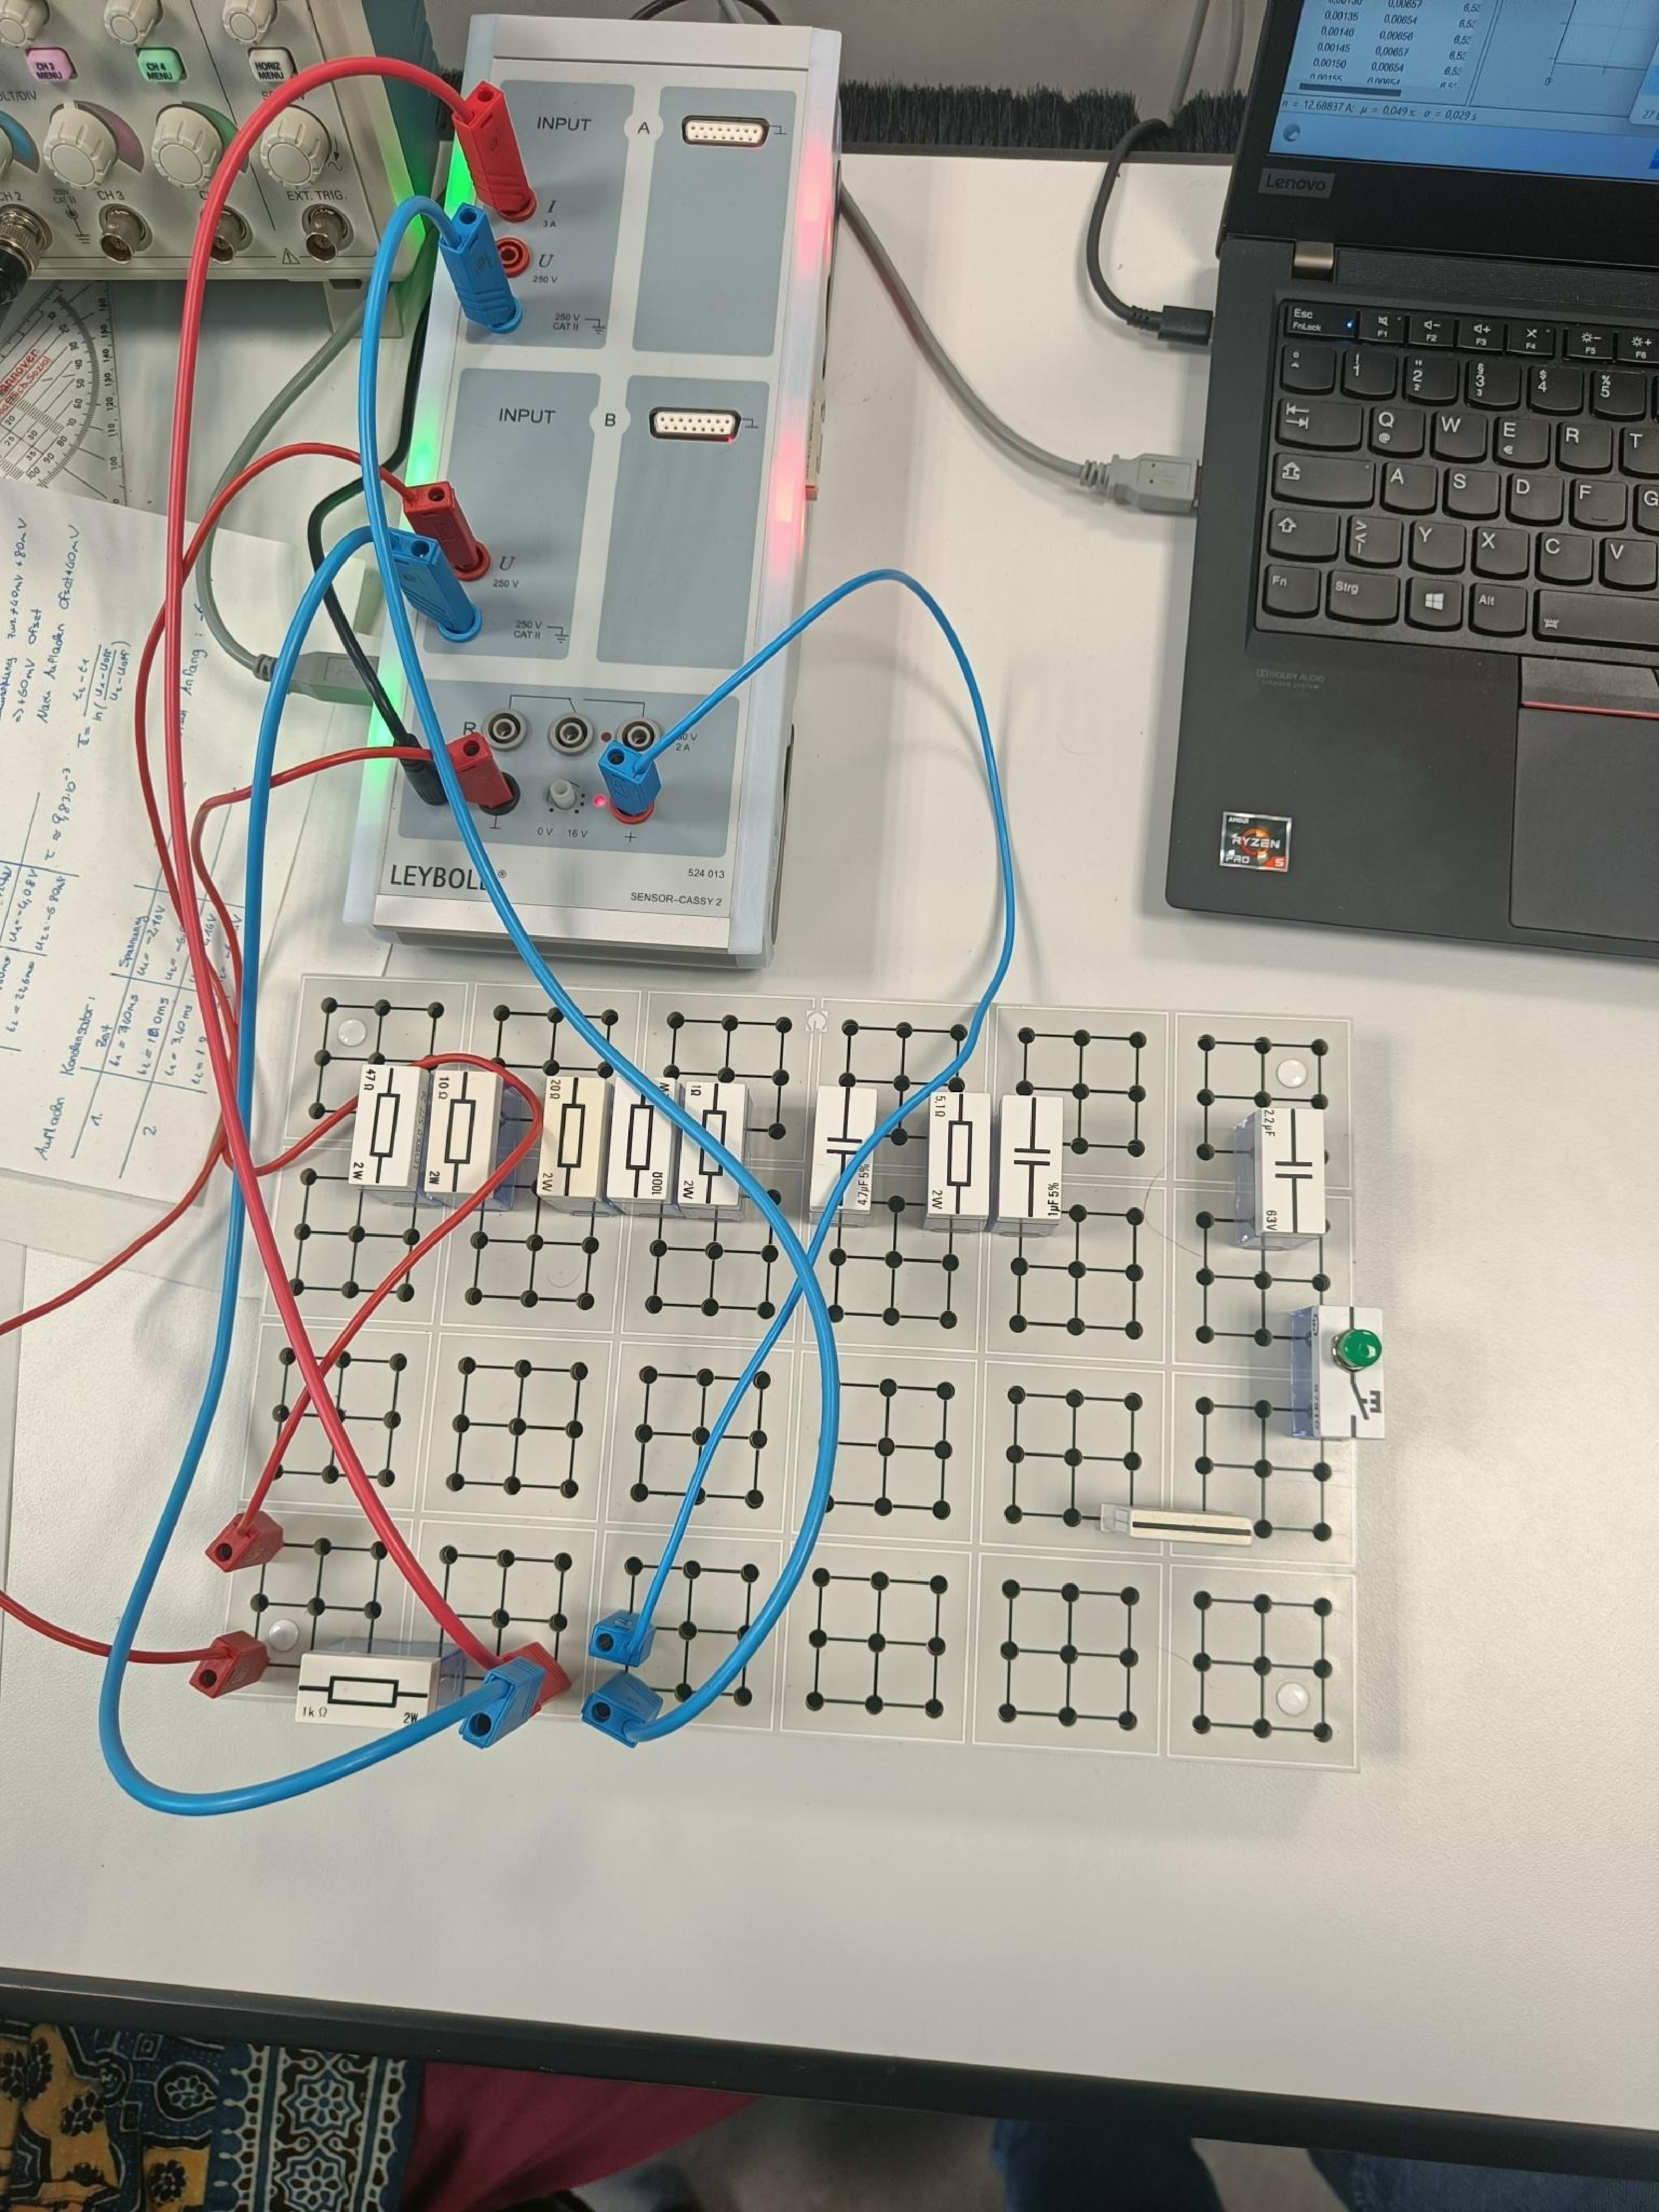
\includegraphics[width=0.5\textwidth]{Bilder_Osziloskop/Schaltung_CASSY_R.pdf}
  \caption{Bild der Schaltung zur Bestimmung des Wiederstands mit CASSY}
  \centering
  \end{figure}
  
In dem Bild können Sie unsere Aufgebaute Schaltung sehen, und wie wir das CASSY angeschlossen haben. \\
   
Aus der Leistungsgrenze des Wiederstands und der maximalen Stromstärke des CASSY konnten wir schließen, dass wir an diesem Maximal 10V anlegen dürfen. Deshalb haben wir das Cassy auf 9V geregelt. 
Als Intervall welches CASSY uns anzeigt haben wir -10V-10V verwendet. 
Aufgrund unseres großen Wiederstands, fließen rellativ geringe Ströme. 
Bei unserer Ersten Testmessung hatten wir ein zu großes Stromintervall gewählt, weshalb der Digitalisierungsfehler die Messung dominiert hat. Deshalb haben wir das kleinste Intervall für den Strom verwendet. 
 Für die Messung haben wir keinen Trigger verwendet, sondern haben diese manuell gestartet. Hierführ haben wir nur das Messintervall und die Messzeit eingestellt. \\
 Zunächst haben wir eine Testmessung durchgeführt die wir manuel gestartet und gestopt haben, um zu sehen ob wir ein Signal erhalten. 
Diese Messung konnten wir auch verwenden um unsere Messzeit sinnvoll ein zu stellen. 
 

 Wir wollen sicherstellen, dass der statistische Fehler auf die Strom und Spannungsmessung kleiner ist als der Fehler aufgrund der Digitalisierung. 
 Da dieser durch mehr Messpunkte verkleinert werden k ann, wärend der Digitalisierungsfehler gleich bleibt.
 Dafür haben wir erst kurz überschlagen, wie groß der Digitalisierungsfehler ist. Daraus konnten wir bestimmen wieviele Messpunkte wir Mindestens brauchen um darunter zu liegen. 
 
 \begin{equation}
  \sigma_D = \frac{Itervall}{2^{12}*\sqrt{12}}
 \end{equation}
 
 Die $2^{12}$ kommt aus der Digitalisierungsrate des CASSY und die $\sqrt{12}$ aus der Annahme, dass dieser Fehler gleichferteilt ist. 
 
 Desweiteren wissen wir, dass der Statistischen Fehler auf den Mittelwert mit $ \bar{\sigma} = \frac{\sigma}{\sqrt{N}}$ bestimmt wirt.
 Dabei ist $\sigma$ die Standardabweichung zu der Verteilung unserer Messdaten.
 Diese können wir in CASSY Lab 2 mit einem Gauß fit grob bestimmen, und verwenden um ein Mindestwert für unsere Messwertanzahl N zu berechnen.
 Dabei fordern wir $\sigma_D > \bar{\sigma}$. Daraus konnten wir die Mindestanzahl von Messpunkten die wir benötigen auf ca. 500 bestimmen.
 
\begin{table}[H]
        \centering
        \begin{tabularx}{1\textwidth}{X X X X} % adjust width as needed
            \toprule
            \textbf{Intervall} & \textbf{Messzeit} & \textbf{Trigger} & \textbf{Spannungs/Strom-intervall} \\
            \midrule
            50$\mu$s  & 0.1s & -- & -10V - 10V \\
            \textbf{Messwerte:}& $\Rightarrow$ N = 2001& & -0.01A - 0.01A\\
            \bottomrule
        \end{tabularx}
        \caption{Messwertserfassungseinstellungen des CASSY}
        \label{tab:mytable}
    \end{table}

Wir haben uns entschieden Einstellungen zu verwenden, die wir Problemlos auch für die Messung der Auf/Entladung des Kondensators verwenden können. Weswegen wir die Messzeit auf ca. zehn $\tau$ gewählt haben. 

Nachdem wir alle Einstellungen im CASSY vorgenommen hatten, starteten wir eine Testmessung. Bei dieser konnten wir erkennen, dass die Spannung und der Strom um einen Wert (ungefähr der eingestellte) fluktuiert. 
Da dies unseren Erwartungen entsprochen hat, haben wir unsere tatsächliche Messung gestartet. 

Hierführ haben wir eine Spannung mit dem CASSY Eingestellt. Eine Messung durchgeführt, und die Daten gespeichert. Dies haben wir insgesamt für 10 verschiedene Spannungswerte gemacht. \\

Im folgenden haben wir sämtliche Graphen, und Zahlenwerte mit hilfe des 
programms "Cassy\_ Wiederstand.py"\ ermittelt und aus diesem übernommen. 
 
\subsection{Diskussion der Ergebnisse}
Hier kann man die Häufigkeitsverteilung der einzelnen gemessenen Spannungen und Stromstärken sehen.
Dabei hatten wir in dieser Messung eine Spannung von 3.97V angelegt.
Dabei fällt auf, das das Cassy nicht nur einen Spannungswert misst, sondern eine leichte Schwankung um diesen.
Gleichges gilt für die Stromstärke.


  \begin{figure}[H]
      \centering
      \includegraphics[width=0.7\textwidth]{plots/messung-wiederstand-07.pdf}
      \caption{Verteilung der gemessenen Spannung und Stromstärke bei einer angelegen Spannung von 3.97V}
  \end{figure}
  
\subsubsection{statistischer Fehler auf die Messungen} 
Bei genauerer Betrachtung fällt auf, das sowohl Spannung wie auch Stromstärke einer Gaußverteilung folgen.
Für die weitere Auswertung haben wir für jede Messung immer den Mittelwert und die Unsicherheit auf den Mittelwert berechnet.

Für die Berechnung des Mittelwerts können wir folgenden Zusammenhang benutzen. 

\begin{equation}
	\bar{x} =\frac{1}{N} \sum_{i = 1}^N x_i
\end{equation}

Wobei N die Anzahl unserer Messpunkte ist, in unserem Fall 2001 und $x_i$ der Wert der einzelnen Messpunkte. Diesen Mittelwert müssen wir für alle unsere Strom und Spannungsmessungen bestimmen. 
Mit diesem können wir den Fehler auf den Mittelwert bestimmen. 

\begin{equation}
	\sigma^2 = \frac{1}{N-1} \sum_{i = 1}^N (x_i - \bar{x})^2  \Rightarrow \bar{\sigma} = \frac{\sigma}{\sqrt{N}}
\end{equation}

Hier ist $\sigma$ die Standardabweichung auf den Einzelwert, und $\bar{\sigma}$ der Fehler auf den Mittelwert.

Desweiteren müssen wir den Digitalisierungsfehler in unserem Fall als statistischen Fehler betrachten, und auch bei der Linearen Regression berücksichtigen. 
Somit ergeben sich für den Statistischen Fehler auf die Mittelwerte folgende Werte.

\begin{table}[H]
    \centering
    \begin{tabularx}{1\textwidth}{X X X X} % adjust width as needed
        \toprule
        \textbf{Messung} & \textbf{Mittelwert} & $\pmb{\bar{\sigma}_{Ui}}$ & \textbf{Gesamtfehler stat.} \\
        \midrule
        1 & 9.0V & 0.1mV & 3.8mV \\
        2 & 8.07V & 0.4mV & 15.9mV \\
        3 & 7.07V & 0.1mV & 4.9mV \\
        4 & 5.99V & 0.1mV & 3.3mV \\
        5 & 4.97V & 0.0mV & 2.3mV \\
        6 & 3.97V & 0.1mV & 5.0mV \\
        7 & 2.95V & 0.1mV & 4.8mV \\
        8 & 8.52V & 0.1mV & 3.4mV \\
        9 & 7.53V & 0.0mV & 2.3mV \\
        10 & 6.53V & 0.1mV & 4.0mV \\
        \bottomrule
    \end{tabularx}
    \caption{Spannungen mit Fehlern}
    \label{tab:mytable}
\end{table}
\begin{table}[H]
    \centering
    \begin{tabularx}{1\textwidth}{X X X X}
        \toprule
        \textbf{Messung} & \textbf{Mittelwert} & $\pmb{\bar{\sigma}_{Ii}}$ & \textbf{Gesamtfehler .stat} \\
        \midrule
        1 & 9.0mA & 341.0nA & 1.4mA \\
        2 & 8.1mA & 493.0nA & 1.4mA \\
        3 & 7.1mA & 339.0nA & 1.4mA \\
        4 & 6.0mA & 329.0nA & 1.4mA \\
        5 & 5.0mA & 332.0nA & 1.4mA \\
        6 & 4.0mA & 339.0nA & 1.4mA \\
        7 & 3.0mA & 341.0nA & 1.4mA \\
        8 & 8.6mA & 337.0nA & 1.4mA \\
        9 & 7.6mA & 331.0nA & 1.4mA \\
        10 & 6.6mA & 331.0nA & 1.4mA \\
        \bottomrule
    \end{tabularx}
    \caption{Stromstärken mit Fehlern}
    \label{tab:mytable}
\end{table}
Der Gesamtfehler berechnet sich dabei aus der quadratischen Addition von statistischem Fehler auf den Mittelwert und dem Digitalisierungsfehler.
Wie zu sehen ist, ist der Fehler auf den Mittelwert bei der Spannung sowie bei der Stromstärke deutlich kleiner als der Digitalisierungsfehler.\\

\subsubsection{Lineare Regression}

Mit der Methode der kleinsten Quadrate, kann aus den berechneten Mittelwerten und deren Fehler nun eine Lineare Regression auf unsere Daten angepasst werden.
Im oberen Graphen sind die Mittelwerte von Spannung und Strom gegeneinander aufgetragen.
Die grüne Gerade ist die Anpassung einer Geraden an die Wertepaare.
 
Der untere Plot stellt dar, wie weit die Mittelwerte von der Linearen Regression abweichen.  
Die Lineare Regression haben wir mit dem program (...) durchgeführt.\\

Den Fehler auf die Spannung im unteren Residualplot haben wir wie folgt berechnet:
\begin{equation}
    \sigma_{U-Resultierend} = \sqrt{(R \sigma_I)^2 + (\sigma_U)^2}
\end{equation}

 \begin{figure}[H]
  \centering
  \includegraphics[width=1\textwidth]{plots/lineare_regression_alle.pdf}
  \caption{Lineare Regression mit allen Messungen}
  \centering
  \end{figure}


Im Residualplot ist zu sehen, das unsere Messwerte um die linare Regression streuen, dabei liegt die Lineare Regression, in den meisten Fällen im Rahmen des Fehlers.
Dem unteren Graphen kann man ebenfalls entnehmen, dass hier keine Systematiken vorliegen. 
Zu bemerken ist, dass der im unteren Residuen Plot letzte Messwert, stark ausbricht. Weshalb wir diesen im folgenden exkludieren werden, um die Genauigkeit unseres Ergebnis zu erhöhen.

Der Außreißer ist die Messung bei 9V. Beim analysieren unserer Rohdaten fällt auf, dass auch unsere Testmessungen, welche wir bei 9V durchgeführt hatten, ebenfalls alle  nach oben ausgerissen sind, wenn wir diese in der Linearen Regression mitbeachtet haben.\\
Dies könnte daran liegen, dass der Wiederstand sich bei dieser Spannung aufheizt, und somit größer wird, als sein eigentlicher Wert. 
Da der Messvorgang jedoch nicht lange dauerte, und die 9V unsere erste Messung waren, also sich zu dem Zeitpunkt der Wiederstand am wenigsten aufgeheizt haben sollte ist es eher unwarscheinlich, dass die starke Abweichung daher kommt. \\

Ein weiterer Grund die Messung bei 9V herraus zu nehmen liefert das $\frac{\chi^2}{ndof}$ Wobei hier "ndof"\ für die Anzahl der Freiheitzsgrade steht.

\begin{equation}
ndof = N_{Werte} - N_{Parameter}
\end{equation}

in unserem Fall haben wir 10 Werte und 2 Parameter in der Linearen Regression.

Das $\chi^2$ ist dabei gegeben als:

\begin{equation}
	\chi^2 = \sum_{i=1}^N \frac{(U_i - (RI_i + b))^2}{\sigma_{Ui}^2+(R\sigma_{Ii})^2}
\end{equation}

Hier steht $ U_i , I_i $ für die Mittelwerte der einzelnen Messungen und R für den aus der Linearen Regression bestimmten Wiederstand. 
Das b stammt ebenfalls aus der Linearen Regression, und bezeichnet den U-Achsen Abschnitt unserer Anpassung. Dieses ist jedoch sehr klein, was zu erwarten war.
 
$\frac{\chi^2}{ndof}$ ist ein Maß für die Qualtät der Anpassung.  
Für das $\chi^2$ mit und ohne den Wert bei 9V ergibt sich:

\begin{table}[H]
    \centering
    \begin{tabularx}{1\textwidth}{X X X X}
        \toprule
         & \textbf{Freiheitsgrade} & $\pmb{\frac{\chi^2}{ndof}}$ & \textbf{b} \\
        \midrule
        Alle Messungen: & 8 & 2.509 & 0.0002V \\
         bereinigt & 7 & 0.807 & 0.0027V \\

        \bottomrule
    \end{tabularx}
    \caption{Qualität der Anpassung}
    \label{tab:mytable}
  \end{table}

Hier können wir sehen, dass die Quallität der Anpassung sich deutlich verbessert, wenn wir die Messung bei 9V aus der Auswertung nehmen.
 
 \begin{figure}[H]
  \centering
  \includegraphics[width=1\textwidth]{plots/lineare_regression_final.pdf}
  \caption{Lineare Regression ohne Messung bei 9V}
  \centering
  \end{figure}

Hier können wir sehen, dass die Lineare Regression nun im Rahmen beinahe aller Messfehler liegt und keine Systematik vorliegt.
In dem oberen Plot sind ebenfalls Fehlerbalken, diese sind jedoch nicht zu sehen, da sie im Vergleich zu der Skalierung sehr klein sind.\\

Bei einer guten Anpassung erwarten wir ein  $\frac{\chi^2}{ndof}$ von ungefähr 1. Unser Wert von 0.807 ist etwas kleiner, was darauf schließen lässt, dass wir unsere Fehler überschätzt haben. 
 
Da wir jedoch nur 9 Datenpunkte haben, und somit 7 Freiheitsgrade ist $\frac{\chi^2}{ndof} = 0.807$ ein gutes Ergebniss. 

Aus der Steigung der Geraden, der Linearen Regression können wir nun den Wiederstand bestimmen. Aus der linearen Regression erhalten wir ebenfalls den statistischen Fehler auf R.
 Dieser ergibt sich zu:\\

{\centering R = (995.5 $\pm$0.283$_{stat}$)$\Omega$ \par} 


\subsubsection{Systematische Fehler}
Bei der Berechnung der Systematischen Fehlern haben wir die Verschiebemethode gewählt.
Dafür haben wir Stromstärken und Spannungswerte um den Systematischen Fehler verschoben, d.h:
\begin{equation}
    \sigma_{U_i,Systematisch}=\frac{(0.01U_i+ 0.005 * U_{Bereichswert})}{\sqrt{3}}
\end{equation}
\begin{equation}
    U_{i,verschoben} = U_i \pm \sigma_{U_i,Systematisch}
\end{equation}
\begin{equation}
    \sigma_{I_i,Systematisch}=\frac{(0.02I_i+ 0.005 * I_{Bereichswert})}{\sqrt{3}}
\end{equation}
\begin{equation}
    I_{i,verschoben} = I_i \pm \sigma_{I_i,Systematisch}
\end{equation}
Mit diesen verschobenen Werten haben wir erneut die Lineare Regression durchgeführt.
Den Systematischen Fehler von U auf R haben wir mit folgender Formel berechnet:
\begin{equation}
    \Delta R_{U+} = \frac{1}{2} (|R_{U+} - R| + |R_{U-} - R|)
\end{equation}
Das gleiche haben wir für den Systematischen Fehler von I auf R gemacht.
Anschließend haben wir die systematischen Fehler quadratisch addiert, um den Gesamtsystematischen Fehler auf R zu erhalten.
Dieser war $R_{Systematisch} = 12.9\Omega$. \\
 
Damit ergibt sich:
\centering{R = $(995.5 \pm 0.3_{stat} \pm 12.9_{syst}) \Omega$}

\end{aufgabe}


\begin{aufgabe}{Lade- und Entladekurven des Kondensators mit dem Oszilloskop}
  Beschreiben Sie den Versuchsaufbau unter Verwendung eines
  Schaltbildes. Beschreiben Sie die Versuchsdurchführung unter Angabe
  der relevanten Messwerterfassungseinstellungen. Zeigen Sie für den
  Lade- und den Entladevorgang jeweils ein Bild der gemessenen
  Spannungsverläufe auf dem Oszilloskopschirm. Lesen Sie mithilfe der
  Cursor jeweils die Zeitkonstante ab. Berechnen Sie den gewichteten
  Mittelwert der Zeitkonstanten. Berechnen Sie daraus die Kapazität
  und geben Sie sie mit statistischer und systematischer
  Messunsicherheit an.
  
\subsection{Aufbau der Messung mit Osziloskop}  
   
  Für diesen Teil des Gesamtversuchs benötigen wir folgende Geräte:\\
  
  \textbf{Verwendete Geräte:}
  \begin{itemize}
  	\item TDS 200 4B Oszilloskop
  	\item Sensor CASSY 2
  	\item Rastersteckplatte DINA A4
  	\item 10 $\mu$F Kondensator
  	\item 1 k$\Omega$ Wiederstand
  	\item Brückenstecker
  	\item 3 Kabel rot / blau
  	\item Taster
  \end{itemize}   

  Wir haben uns entschieden den gesamten Versuch mit einem 10$\mu$F Kondensator und einem 
  1 k$\Omega$ Wiederstand durch zu führen. Hierfür haben wir uns entschieden, da wir so
  eine größere Zeitkonstante erhalten. Dies ist erwünschenswert, da der 
  Lade/Entlade Vorgang so langsamer verläuft. Somit haben wir eine Höhere Auflösung 
  der Messungen dies verringert den Messfehler. Allerdings führt dies auch dazu, dass nur wenig
  Strom durch den Wiederstand fließt. Ein großer Wiederstand erhöht also auch den Fehler auf 
  den Strom den wir später mit dem Sensor CASSY messen, da dieses nicht beliebig kleine 
  Ströme messen kann. Hier ist ein größeres $\tau$ (Zeitkonstante) jedoch über eine größere
  Genauigkeit des Stroms zu wählen. Noch größere Wiederstände hätten jedoch keinen Sinn ergeben, 
  da so der Strom nicht mehr gut messbar gewesen wäre.
  
  \subsection{Durchführung der Messung mit Oszilloskop}  
  
  \begin{figure}[H]
  \centering
  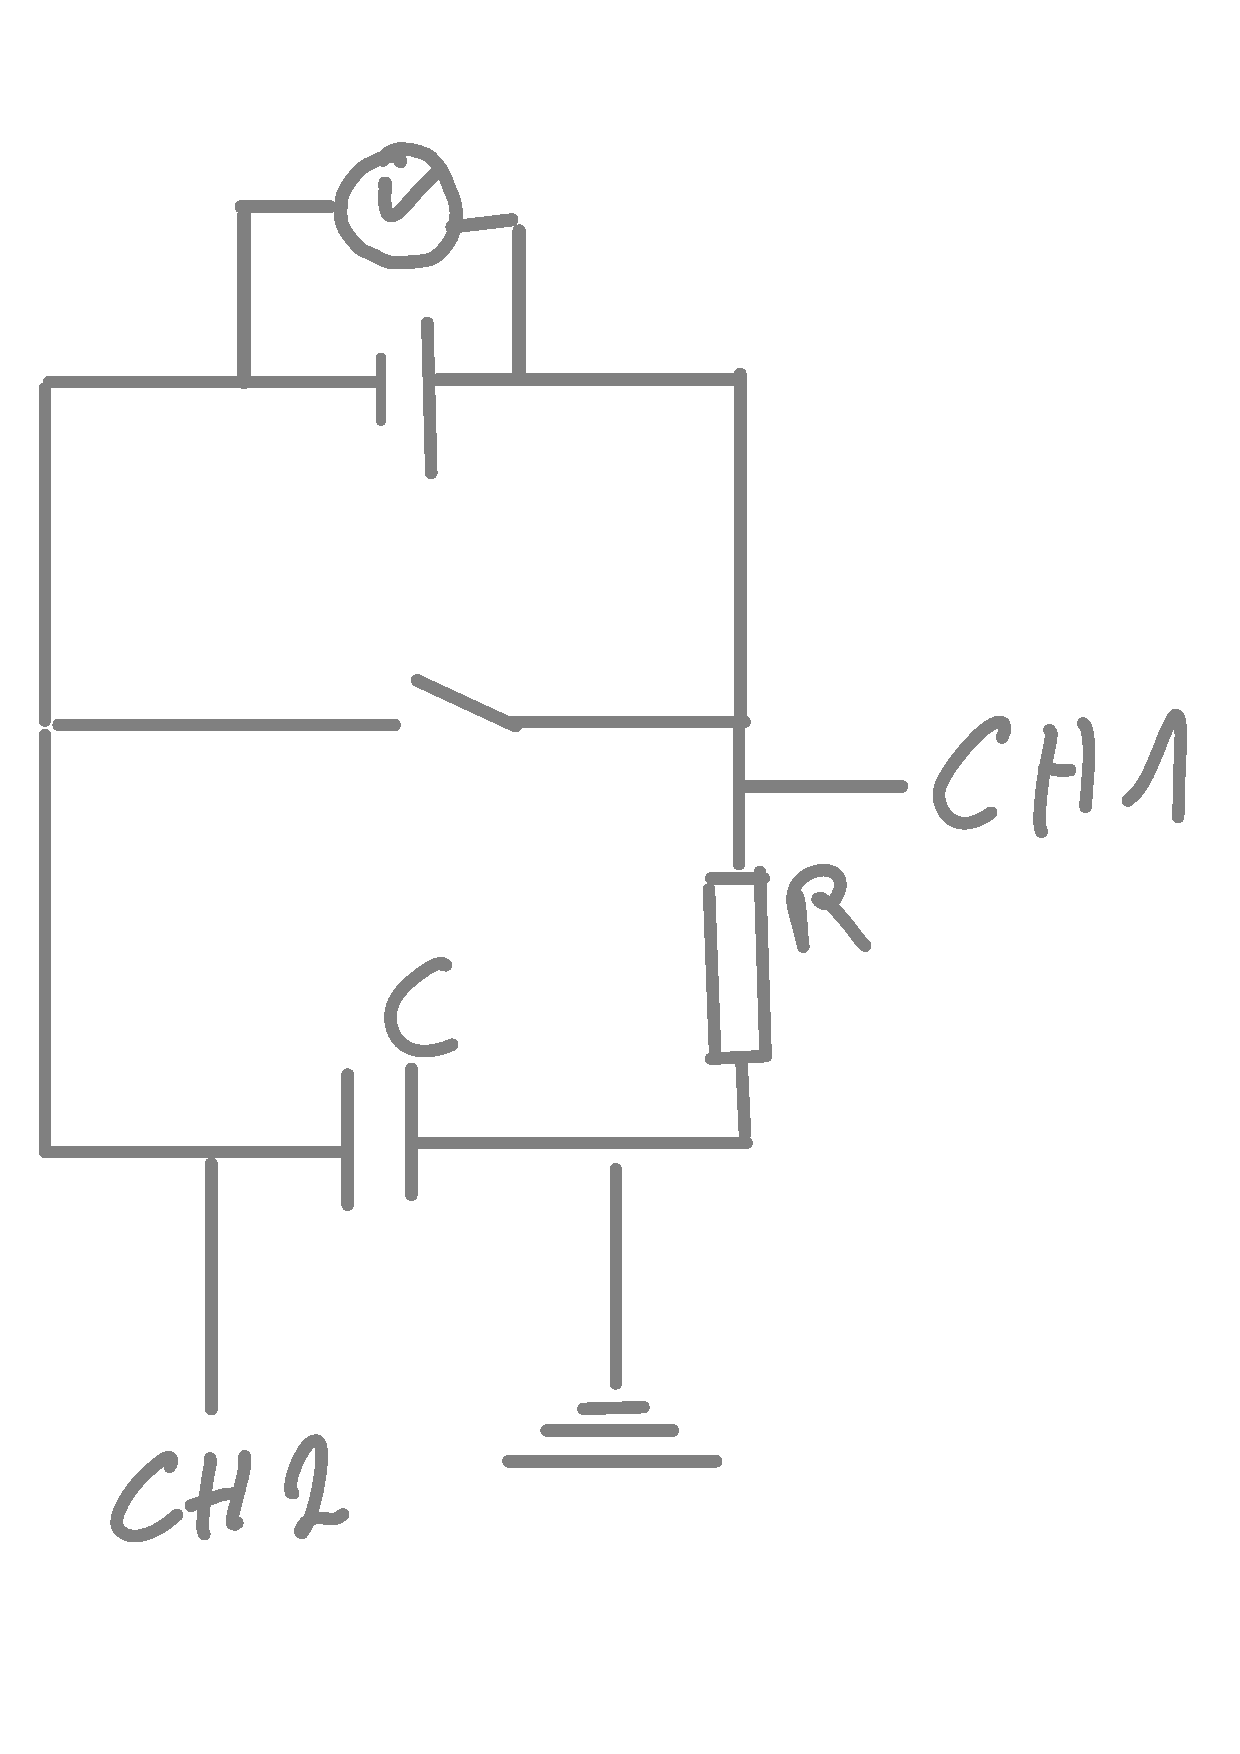
\includegraphics[width=0.5\textwidth]{schaltzkisse-osziloskop.pdf}
  \caption{Schaltplan Oszilloskop}
  \centering
  \end{figure}

  In der obigen Skizze können Sie das Schaltbild zu dem Versuch sehen. 
  Auf dem Steckbrett werden hierfür Kondensator und Wiederstand in Reihe gesteckt.
  Parallel zu dem Kondensator wird ein Schalter eingebaut, der bei bedarf den Stromkreis
  schließen bzw. öffnen kann. Ebenfalls paralell wird eine Spannungsquelle angeschlossen. 
  Hier wird das Sensor CASSY als Spannungsquelle verwendet. Wir haben außerdem noch mit dem
  Sensor CASSY die angelegte Spannung gemessen. An diese Schalltung wird das
  Oszilloskop angeschlossen. Für beide Channel wurde die gleiche Masse verwendent, welche zwischen Kondensator und Wiederstand angeschlossen war.
  Chanel 1 \& 2 werden wie im Schaltbild angeschlossen.
  So wird auf CH2 die Spannung die über den Kondensator abfällt gemessen, und 
  auf CH1 die Spannung die über den Wiederstand abfällt. 

  \begin{figure}[H]
  \centering
  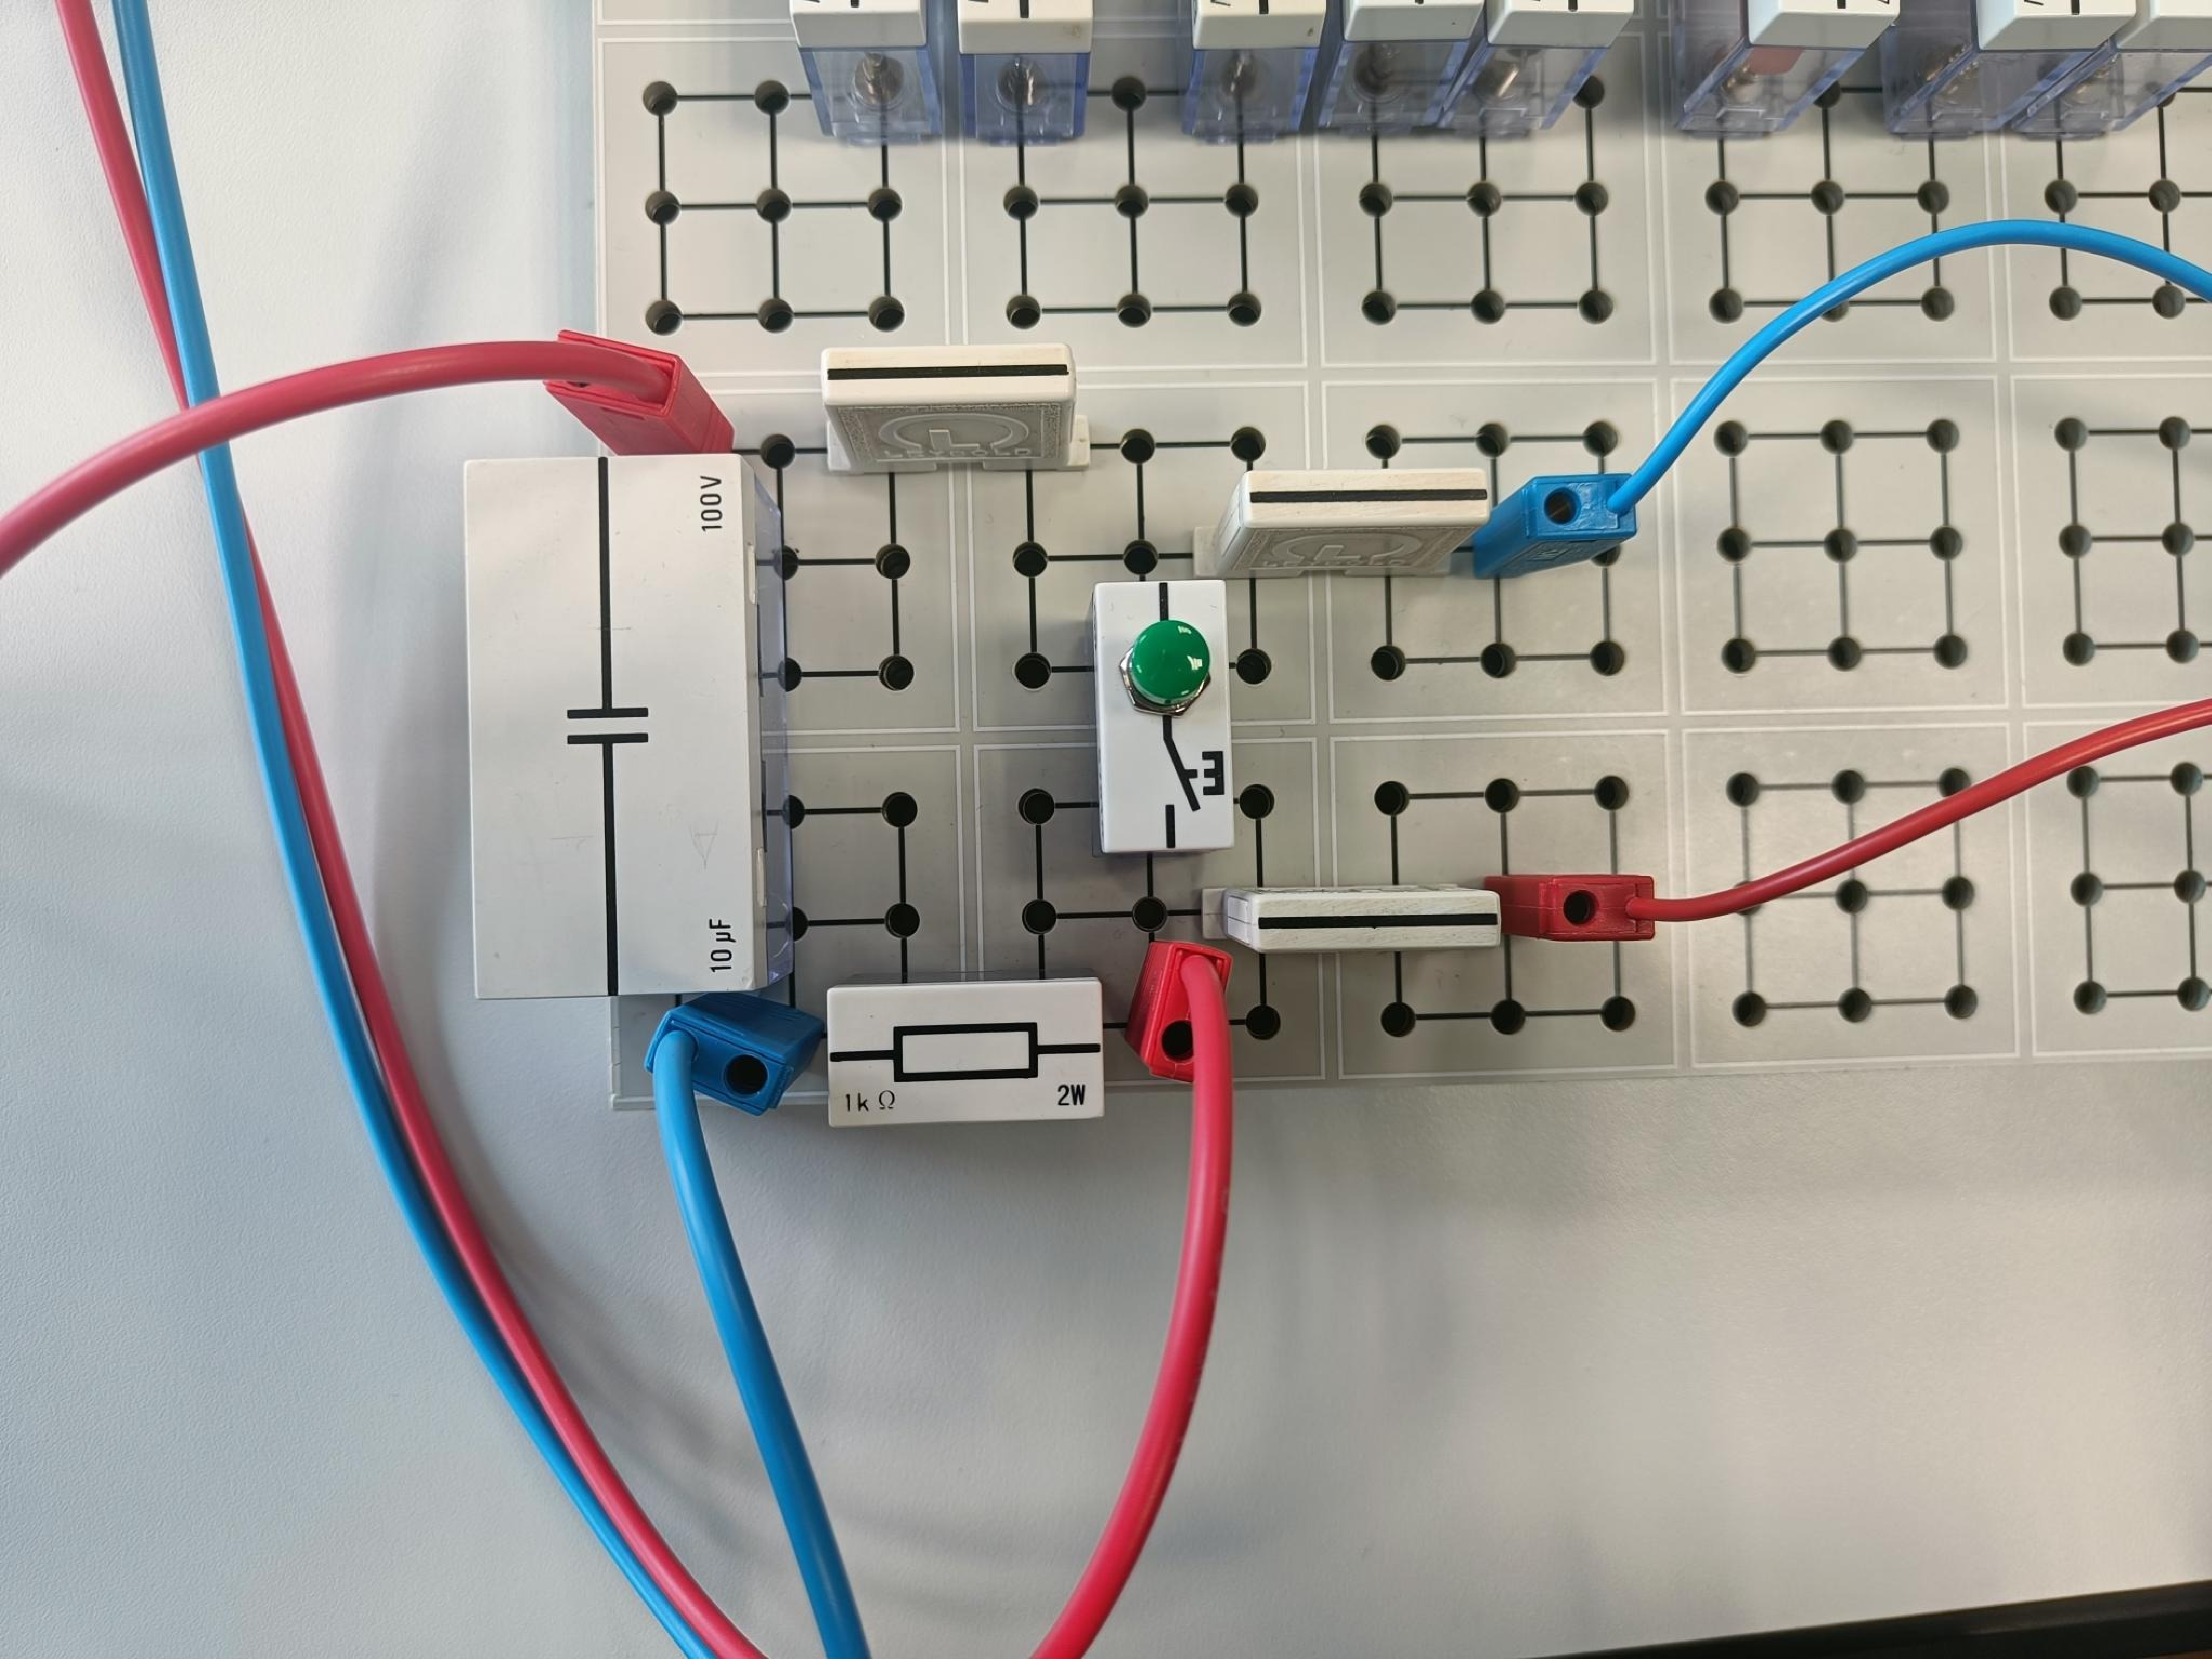
\includegraphics[width=0.5\textwidth]{Bilder_Osziloskop/Schaltung_Osziloskop_02.pdf}
  \caption{Bild der Schaltung}
  \centering
  \end{figure}
 
  Bei der Versuchsdurchführung haben wir wie im Aufbau bereits beschrieben den Versuch 
  aufgebaut. Um die Spannung ein zu stellen und die Auflösung des Oszilloskop richtig zu
  wählen, haben wir das Sensor CASSY verwendet um die Eingangsspannung zu bestimmen. \\
  Da unser Wiederstand eine Leistungsgrenze von 2W hat, und das CASSY maximal 0.1A liefert, muss die Spannung unter 10V liegen.
  Um die maximale Auflösung des Oszilloskops auszunutzen, sollte das Signal den gesamen Werteberich auf dem Bildschirm ausfüllen.
  Die Einstellung der y-Achse mit Darstellung bis 8V lag am dichtesten unter 10V. 
  Um auch kleine schwankungen nach oben noch aufzeichnen zu können, haben wir 7.1V gewählt. \\
  Zur Einstellung des Oszilloskops haben wir zunächst die Entladung des Kondensators betrachtet. 
  
  \subsubsection{entladen des Kondensator}
  
  Hierfür haben wir den Trigger auf CH2 auf 7.00V 
   steigende Flanke gestellt. Steigende Flanke ist hier sinnvoll, da auf Grund der Polung 
  die Spannung am Kondensator negativ ist. Somit steigt die Spannung asymtotisch zu null. 
  Zum starten der Messung haben wir den in der Schaltung verbauten Taster betätigt.
  So konnten wir eine erste Entladung aufzeichnen. Hierraus konnten wir dann die Restlichen 
  Einstellungen schließen. Ziel war es, möglichst viel vom Entladevorgang auf zu zeichnen, und 
  einen kurzen Zeitraum vor dem Entladen.
  wir haben die Zeiteinstellungen so gewählt, dass 5 $\tau$ auf unserem Bildschirm angezeigt
  werden. So sind wir sicher gegangen, dass wir nur den relevanten teil der Entladung aufzeichnen, 
  und nicht die Zeitspanne in welchem die Spannungen asymtotisch gegen null streben. 

\begin{figure}[H]
  \centering
    \includegraphics[width=0.7\textwidth]{Bilder_Osziloskop/Triggermenü_Osziloskop.pdf}
  \caption{Triggermenü des Oszilloskops}
  \centering
\end{figure}

Oben sehen sie ein Bild des Triggermenüs des Osziloskops. Hier haben wir sämtliche Triggereinstellungen für das Messen des Entladens eingestellt.
Hier sieht man auch, dass wir das Signal von CH2 invertiert haben, um dieses angenehmer
auf dem Bildschirm darstellen zu können. So konnten wir außerdem den Nullpunkt der beiden 
Spannungsverläufe optisch an die ungefähr gleiche Stelle legen. Der folgenden Tabelle
können sie die Einstellungen entnehmen die wir am Oszilloskop vorgenommen haben.
Diese Einstellungen sind spezifisch für den Entladevorgang.


\begin{table}[H]
        \centering
        \begin{tabularx}{0.8\textwidth}{X c c c c} % adjust width as needed
            \toprule
            \textbf{Chanel} & \textbf{Kästchen} & \textbf{M} & \textbf{Trigger} & \textbf{Flanke} \\
            \midrule
            CH1 & 1.00V & 5.00ms & -- & -- \\
            CH2 & 1.00V & 5.00ms & 7.00V & positiv \\
            \bottomrule
        \end{tabularx}
        \caption{Übersicht der Einstellungen am Oszilloskop}
        \label{tab:mytable}
    \end{table}

Wir haben die Messung der Entladung mit unseren neuen Einstellungen wiederholt. Um zu überprüfen ob diese passen und reproduzierbar sind.

 


\begin{figure}[H]
  \centering
    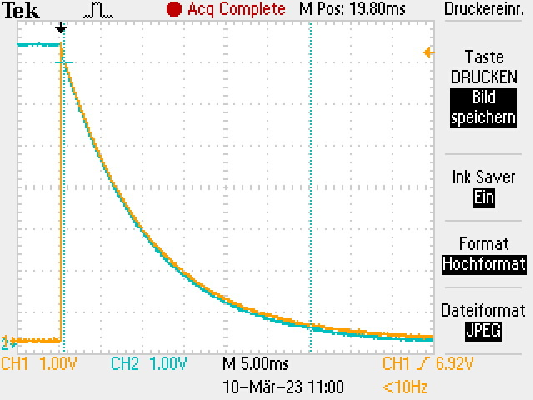
\includegraphics[width=0.7\textwidth]{Bilder_Osziloskop/Entladen_Kondensator_02.pdf}
    \caption{Endlade Vorgang vom Wiederstand und dem Kondensator}
  \centering
\end{figure}
Oben Abgebildet ist der Spannungsverlauf am Kondensator (blau) und am Wiederstand (orange) während des Entladens.
Hier ist zu beachten, das Channel 2 (der Kondensator) invertiert ist in der Darstellung.
Dies haben wir gemacht, damit wir die Nulllinien angenehm aufeinander legen können.
Diese Entladekurven ensprechen dabei unserer Erwartung, da die Spannung am Kondensator abnimmt und die Spannung am Wiederstand anfangs groß ist, und dann gegen 0 läuft.
Nach Augenmaß verlaufen diese auch beide Exponentiell, was den in den Grundlagen beschriebenen Entladevorgang entspricht.

Zur bestimmung von $\tau$ haben wir bei der Entladung insgesamt 4 Messungen durchgeführt. 
Jewails 2 für Kondensator und Wiederstand. Dies haben wir getan um zu überprüfen ob unsere Messungen reproduzierbar waren. 
Und um sicher zu gehen, dass unsere Messung kein Ausreißer sind. 


Bei unseren Bildern vom Osziloskop haben wir diese mit der Osziloskop eigenen Funktion gemacht.
Deshalb ist der Wert der Cursor auf den Bilder nicht mehr zu sehen, was uns erst im nachhinein aufgefallen ist.
Wir haben aber alle Messwerte auf unsrem Messprotokoll notiert.

\begin{figure}[H]
  \centering
    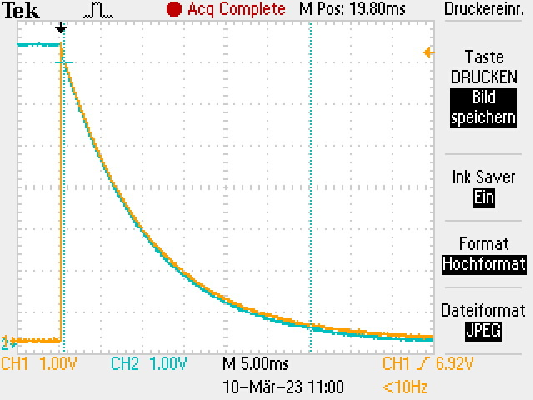
\includegraphics[width=0.7\textwidth]{Bilder_Osziloskop/Entladen_Kondensator_02.pdf}
    \caption{Endlade Vorgang vom Wiederstand und dem Kondensator}
  \centering
\end{figure}
Oben Abgebildet ist der Spannungsverlauf am Kondensator (blau) und am Wiederstand (orange) während des Entladens.
Hier ist zu beachten, das Channel 2 (der Kondensator) invertiert ist in der Darstellung.
Diese Entladekurven ensprechen dabei unserer Erwartung, da die Spannung am Kondensator abnimmt und die Spannung am Wiederstand anfangs groß ist, und dann gegen 0 läuft.
Nach Augenmaß verlaufen diese auch beide Exponentiellen, was den in den Grundlagen beschriebenen Entladevorgang entspricht.

\subsubsection{Bestimmung des Ofset}
Zum bestimmen des Offsets für die Entladung des Kondensator haben wir sowohl den Wert der Asymptote bestimmt, wie auch die Rauschspannung am Wiederstand.
Um den Wert der Asymptote zu bestimmen, haben wir die dargestellte Zeit auf 10 $\tau$ vergrößert, da man mit dieser Einstellung schon in einen Bereich kam, wo die Spannungswerte am Kondensator nicht mehr abgenommen haben, sodern geschwankt sind.
Wir haben dann den Mittelwert der beiden Spannungswerte genommen, um die es geschwankt ist, da sie näherungsweise gleichverteilt sind.
 
\begin{figure}[H]
     
  \centering
    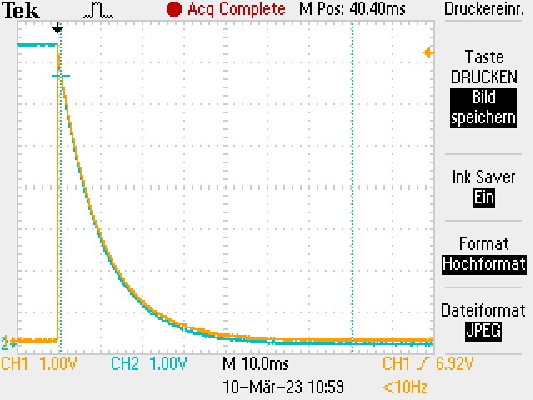
\includegraphics[width=0.7\textwidth]{Bilder_Osziloskop/Entladen_Kondensator_Offset.pdf}
    \caption{Bestimmung des Offsets für die Entladung des Kondensators mit Rauschen}
  \centering
\end{figure}

Hier haben wir auch $U_0$ bestimmt indem wir mit dem Cursor das Signal von CH2 vor dem Begin des Eintladevorgangs abgetastet haben. Daraus ergab sich $U_0 = |7.22V|$ Hier hängt das Vorzeichen von der Polung ab. in unserem Fall war der Kondensator negativ geladen. (Im bild ist CH2 invertiert)
Die Offsetspannung am Wiederstand beim Aufladen des Kondensators haben wir wie für die vorheringen Offsetspannungen die Asymptote bestimmt.

\begin{table}[H]
        \centering
        \begin{tabularx}{1.0\textwidth}{X X} % adjust width as needed
            \toprule
            \textbf{Bauteil} & \textbf{Offset} \\
            Endladen Wiederstand & $U_{off} = 0.04V$ \\
            Endladen Kondensator & $U_{off} = 0.02V$ \\
            Aufladen Wiederstand & $U_{off} = -0.06V$ \\
            Aufladen Kondensator & $U_{0} = -7.22V$ \\
            \midrule
            \bottomrule
        \end{tabularx}
        \caption{Übersicht der Einstellungen am Oszilloskop}
        \label{tab:mytable}
    \end{table}
    
 \subsubsection{Aufladen des Kondensators}
 
 
Für die Messung des Aufladevorgangs mussten wir nur die Trigger Einstellungen ändern sonst konnten wir unsere Einstellungen übernehmen.
In diesem Fall haben wir auch keins der Signale invertiert. 

\begin{table}[H]
        \centering
        \begin{tabularx}{0.8\textwidth}{X c c c c} % adjust width as needed
            \toprule
            \textbf{Chanel} & \textbf{Kästchen} & \textbf{M} & \textbf{Trigger} & \textbf{Flanke} \\
            \midrule
            CH1 & 1.00V & 5.00ms & -- & -- \\
            CH2 & 1.00V & 5.00ms & -80.0mV & positiv \\
            \bottomrule
        \end{tabularx}
        \caption{Übersicht der Einstellungen am Oszilloskop}
        \label{tab:mytable}
    \end{table}
    
Beim messen der Aufladung haben wir zunächst denn Schalter gedrückt und einige Sekunden gewartet, um sicher zu gehen, dass der Kondensator entladen war. 
Dann haben wir den Schalter losgelassen un die Messung ist durch den Trigger automatisch gestartet. 
Hier haben wir ebenfalls erst eine Testmessung durchgeführt, und dann wie beim entladen jeh für Kondensator und Wiederstand 2 Messungen zur bestimmung von $\tau$ gemacht. 

\begin{figure}[H]
  \centering
    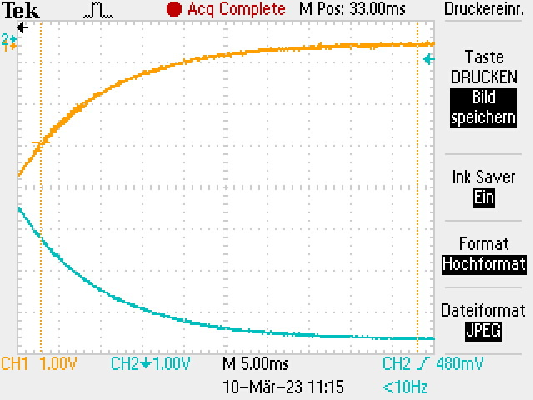
\includegraphics[width=0.7\textwidth]{Bilder_Osziloskop/Aufladen_Kondensator_02.pdf}
    \caption{Aufladen Vorgang vom Wiederstand und dem Kondensator}
  \centering
\end{figure}
Die Abbildung zeigt den Spannungsverlauf von einem typischem Aufladevorgang.
Hier haben wir nichts invertiert, da wir auch so die gleiche Nullline setzen konnten, und trotzdem das gesamte Display zum ablesen nutzen konnten.
Dabei ist allerdings zu beachten das wir die Null ans obere Ende gesetzt haben, da aufgrund von unserer Verkabelung die Spannung am Wiederstand sowie am Kondensator negativ waren, was für die Auswerung allerdings Irrelevant ist.
Die Kondensatorspannung entfernt sich dabei immer weiter von der Nulllinie, und die Spannung am Wiederstand ist macht anfangs einen Sprung und fällt dann gegen Null ab.
Nach augenmaß verlaufen beide Kurven exponentiell, was auch den exponentiellen Gleichungen für den Aufladevorgang entspricht.

\subsubsection{Bestimmung von $\tau$}

Zur bestimmung von Tau haben wir mit dem Cursors je zwei Messwerte abgelesen. 
Mithilfe der Formeln die wir bereits in den Grundlagen eingeführt haben, konnten wir dann die Zeitkonstante bestimmen. 
Diese erhalten wir indem wir den Quotienten von unserem Werte Paar nehmen und dann nach $\tau$ umformen. Daraus ergibt sich:


\begin{equation}
	\tau = \frac{t_2 - t_1}{ln\left(\frac{U_1-U_{off}}{U_2-U_{off}}\right)}	
\end{equation}

Wobei wir hier noch den möglichen Ofset beachten müssen. \\
Die obige Formel können wir jedoch nicht für den Aufladevorgang des Kondensators verwenden, wenn wir an diesem den Spannungsabfall messen, da die Funktion die diesen beschreibt von der Form $ y = 1 - e^x $ ist. 
In diesem Fall erhalten wir für die Zeitkonstante:
 
 \begin{equation}
 \tau = \frac{t_2 - t_1}{ln\left(\frac{U_0 - U_1}{U_0 - U_2}\right)}
\end{equation}

Somit können wir Die Zeitkonstante für unsere Messungen bestimmen. Auf Grund der ablesegenauigkeit kommt jedoch auf diesen noch ein Fehler.  \\

 
\begin{figure}[H]
  \centering
    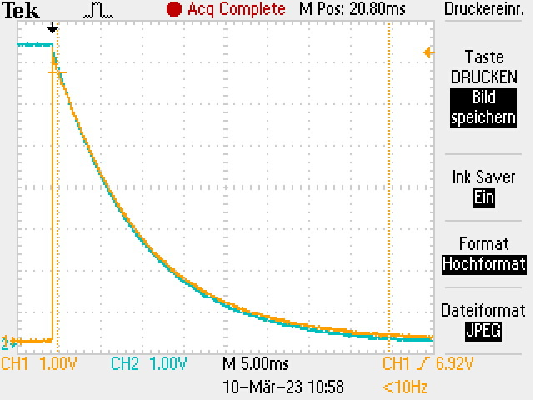
\includegraphics[width=0.7\textwidth]{Bilder_Osziloskop/osziloskop-test-cursor-genauigkeit.pdf}
    \caption{Bestimmung der Genauigkeit des Cursors}
  \centering
\end{figure}


Beim variiren des Cursors um einen Schritt in der Zeit haben wir festgestellt, das die Genauigkeit des Cursors bei 20 $\mu s$ liegt.
Beim Variiren der Spannung haben wir eine Schrittweite des Ablesens von 0.04V festgestellt.
Diese Ableseungenauigkeit muss durch $\sqrt{12}$ geteilt werden, um daraus unseren Fehler auf t und U zu erhalten. 
Dieses lässt sich auch auf alle Auf und Endlademessungen übertragen, da wir immer die gleichen Zoomeinstellungen im Fenster hatten, außer für die Offsetbestimmung. \\
 
Den untenstehenden Rechnungen können sie somit unsere Fehler auf U und t entnehmen. 

\begin{equation}
	\frac{20\quad 10^{-6}s}{\sqrt{12}} = 5.774 \quad 10^{-6}s \qquad  \frac{0.04V}{\sqrt{12}} = 0.0115V 
\end{equation}


Für die Bestimmung des Fehlers auf $\tau$ haben wir den Fehler auf grund der ablesegenauigkeit statischtisch angenommen. Wobei wir eine Ungenauigkeit auf das ablesen der Zeit als auch auf die Amplitude haben. Die Fehlerfortplfanzung lautet somit: 

\begin{equation}
	\sigma_{\tau}^2 = \sum_{i,j=1}^n\left[\frac{\partial \tau}{\partial x_i}\frac{\partial \tau}{\partial x_j}\right]_{x=\mu}V_{ij}^2
\end{equation}

Wobei dies die Form für eine Größe mit zwei Variablen ist, diese kann jedoch problemlos auf n Variablen erweitert werden.
Wir gehen davon aus, dass die Warscheinlichkeitsdichte zu unserem Fehler eine Gaußverteilung ist.
Woraus wir schließen können, dass diese unkorreliert sind und sich somit der Fehler auf $\tau$ vereinfacht zu. 

\begin{equation}
	\sigma_{\tau}^2 = \sum_{i=1}^n\left[\frac{\partial \tau}{\partial x_i}\right]^2_{x=\mu}\sigma_{i}^2
\end{equation}

Wobei hier darauf geachtet werden muss, $\tau$ von 4 Variablen abhängig ist $\tau\left(t_1, t_2, U_1, U_2\right)$.
Weshalb hier nach insgesamt vier Variablen abgeleitet werden muss. Jedoch ist der Fehler auf $t_1$, $t_2$ und auf $U_1$ , $U_2$ jewails gleich. Somit ergibt sich für unser spezifisches Problem folgende Form für die Fehlerfortplfanlzung. 

\begin{equation}
	\sigma_{\tau}^2 = \left[\frac{\partial \tau}{\partial t_1}\right]^2\sigma_{t_1}^2 + \left[\frac{\partial \tau}{\partial t_2}\right]^2\sigma_{t_2}^2 + \left[\frac{\partial \tau}{\partial U_1}\right]^2\sigma_{U_1}^2 + \left[\frac{\partial \tau}{\partial U_2}\right]^2\sigma_{U_2.}^2
\end{equation}

Dieser Fehler muss für jede unserer Messungen neu berechnet werden, da die Formel von den jewailigen $t_1, t_2, U_1, U_2$ Abhängt. 
Diese und alle folgenden Rechnungen ,so wie Graphen, haben wir mit dem Programm tau-osziloskop.py erstellt

\subsection{Messdaten des Oszilloskop und Diskussion dieser}
Hier eine Übersicht von unsern finalen Messdaten. Dabei haben wir die Offsets immer vor der ensprechenden Messung bestimmt.
Bei jeder Messreihe haben wir während der Messung $\tau$ überschlagen (ohne Fehler) um zu sehen, ob die Messung sinnvoll ist.
Hier haben wir beim ausrechnen vom Tau den Offset berücksichtigt.
$U_0$ ist hierbei die Spannung, welche wir am Kondensator im Aufgeladenen Zustand mit dem Oszilloskop gemessen haben.

Am Anfang der Messung haben wir uns dafür entschieden, in einem möglichst großem Zeitintervall zu messen, da wir so weniger Unsicherheit auf die Zeit haben, und auch kleine Schwankungen beim Entladen ausgleichen können.
Dabei haben wir darauf geachtet, das der erste Cursor mindestens $ \frac{1}{20} \tau $ nach dem Entlade beginn liegt.
Da wir ein $\tau$ von $10ms$ haben, und unsere Analyse der Rohdaten auf dem Oszilloskop ergeben hat, dass wir dort keine Effekte des Schalters mehr haben, fanden wir dieses eine gute Annahme.
Der Endpunkt der Messung haben wir dabei mindestens 120mV über der Grenzspannung gewählt, damit wir weit von Rauschen entfernt sind.\\
Während der Messung haben wir gemerkt, das bei so kleinen Spannungen an der rechten Intervallsgrenze, die Ableseungenauigkeit der Spannung groß wird.
Wir werden also wengier Messfehler haben, wenn wir in einem kleineren Intervall messen.
Dieses haben wir ab Messung 3 umgesetzt, wobei ab Messung 5 wir beim Lade Vorgang (Messung 5-8) den Startpunkt etwas weiter weg gewählt haben vom Anfangszeitpunkt.

 
\begin{table}[H]
        \centering
        \begin{tabularx}{1.00\textwidth}{l X X X X}
            \toprule
            \textbf{Nr.} & \textbf{Messung} & \textbf{Zeit} & \textbf{Spannung} & $\tau$ \\
            \midrule
            1. & 1. Endladen & $t_1 = 600 \mu s$ & $U_1 = 6.64V$ & $(9.93 \pm 0.24)ms$\\
            & Wiederstand & $t_2 = 40.4 ms $  & $U_2 = 160mV$ & \\
            \midrule
            2. & 2. Endladen     & $t_1 = 600 \mu s$ & $U_1 = 6.44V$ & $(9.93 \pm 0.24)ms$ \\
            & Wiederstand  & $t_2 = 40.4 ms $  & $U_2 = 160mV$ \\
            \bottomrule
            3. & 1. Endladen     & $t_1 = 400 \mu s$ & $U_1 = 6.76V$ & $(9.90 \pm 0.13)ms$ \\
            & Kondensator  & $t_2 = 31.2 ms $  & $U_2 = 320mV$ \\
            \midrule
            4. & 2. Endladen     & $t_1 = 400 \mu s$ & $U_1 = 6.76V$ & $(10.30 \pm 0.13)ms$ \\
            & Kondensator  & $t_2 = 31.2 ms $  & $U_2 = 320mV$ \\
            \bottomrule
            5. & 1. Aufladen     & $t_1 = 4.5 ms  $ & $U_1 = -4.08V$ & $(9.99 \pm 0.11)ms$ \\
            & Wiederstand  & $t_2 = 22.6 ms $  & $U_2 = -720mV$ \\
            \midrule
            6. & 2. Aufladen     & $t_1 = 4.5 ms  $ & $U_1 = -4.08V$ & $(9.69 \pm 0.11)ms$ \\
            & Wiederstand  & $t_2 = 22.6 ms $  & $U_2 = -680mV$ \\
            \bottomrule
            7. & 1. Aufladen     & $t_1 = 3.4 ms  $ & $U_1 = -2.16V$ & $(10.03 \pm 0.09)ms$ \\
            & Kondensator  & $t_2 = 18.0 ms $  & $U_2 = -6.04V$ & $ U_0 = -7.22V$ \\
            \midrule
            8. & 2. Aufladen     & $t_1 = 3.4 ms  $ & $U_1 = -2.16V$ & $(10.03 \pm 0.09)ms$ \\
            & Kondensator  & $t_2 = 18.0 ms $  & $U_2 = -6.04V$ & $ U_0 = -7.22V$ \\
            \bottomrule
        \end{tabularx}
        \caption{Übersicht der Einstellungen am Oszilloskop}
        \label{tab:mytable}
    \end{table}
    

\begin{figure}[H]
  \centering
    \includegraphics[width=0.7\textwidth]{plots/434170_428396_1A3_tau_errorbar.pdf}
    \caption{Tau von allen Messung mit Statistischem Fehler}
  \centering
\end{figure}
Wie in dem Plot zu sehen ist, ist der Fehler auf $\tau$ durch unser kleiner gewähltes Messintervall ab Messung 3 deutlich geringer geworden.
Unser erwartetes $\tau$ von $10ms$ liegt also für alle Messungen, abgesehen von Messung 5, im Rahmen des Messfehlers.
Da dieser deutlich über dem von uns erwarteten Wert liegt, haben wir ihn in der folgenden Rechnung exkludiert.
Der gewichtete Mittelwert ist dann: $\tau = (9.98 \pm 0.044)ms$.\\

Der von uns bestimmte Wiederstand geht hier nur mit einer Statistischen Unsicherheit ein, da egal wie oft man das Experiment am Osziloskop durchführt, sich die Unsicherheit auf ihn nicht ändert.
Dieser ist die Addition von dem Statistischen und Systematischen Fehler vom Versuch der bestimmung des Wiederstandes.
$ R = (995.5 \pm 12.2) \Omega$\\


Um nun die Kapazität mit Unsicherheiten zu berechenen, müssen die Fehler von der Zeitkonstante und dem Wiederstand fortgepflanzt werden.
Dabei stammt der Statistische Fehler auf die Kapazität nur von $\tau$ und der Systematische von $R$.
Für den Statistischen Fehler verwenden wir die Gauss'sche Fehlerfortpflanzung und den Zusammenhang $C = \frac{\tau}{R}$
\begin{equation}
    \sigma C_{Statistisch} = \sqrt{(\frac{\partial C}{\partial \tau})^2 \sigma_{\tau}^2}
\end{equation}
\begin{equation}
    \sigma C_{Statistisch} = \sqrt{(\frac{1}{R})^2 \sigma_{\tau}^2} = 0.045 \mu F
\end{equation}

Für die Systematische Unsicherheit haben wir die linare Fehlerfortpflanzung verwendet.
\begin{equation}
    \sigma C_{Systematisch} = |\frac{\partial C}{\partial R} \sigma_R| = 0.123 \mu F
\end{equation}

Damit ergibt sich für die Kapazität mit Unsicherheiten:
\begin{equation}
    C = (10.027 \pm 0.045_{statistisch} \pm 0.123_{systematisch}) \mu F
\end{equation}
 
\end{aufgabe}

 
 
\begin{aufgabe}{Lade- und Entladekurven des Kondensators mit Cassy}
  Zeigen Sie für den Lade- und den Entladevorgang jeweils ein Bild des
  Spannungsverlaufs am Kondensator und des Lade- bzw.~Entladestroms.
  Korrigieren Sie erforderlichenfalls den Spannungs- und/oder
  Strom-Offset. Transformieren Sie die Rohdaten geeignet in
  logarithmische Größen und bestimmen Sie mittels linearer Regression
  die Zeitkonstante. Beschreiben Sie, wie Sie die Messunsicherheiten
  behandeln. Berechnen Sie das gewichtete Mittel und geben Sie Ihr
  Endergebnis für die Kapazität mit statistischer und systematischer
  Messunsicherheit an.
  
  
  
Für die Bestimmung der Kapazität, betrachten wir mit CASSY wieder den Lade und Entladevorgang des Kondensators. 
Hier ist der Aufbau der Schaltung sehr ähnlich zu der beim Oszilloskop. jedoch muss das CASSY anders angeschlossen werden.
Wir messen außerdem am Wiederstand die Stromstärke, und nicht die Spannung.

  \begin{figure}[H]
      \centering
      \subfloat[Schaltbild für die Messung mit CASSY]{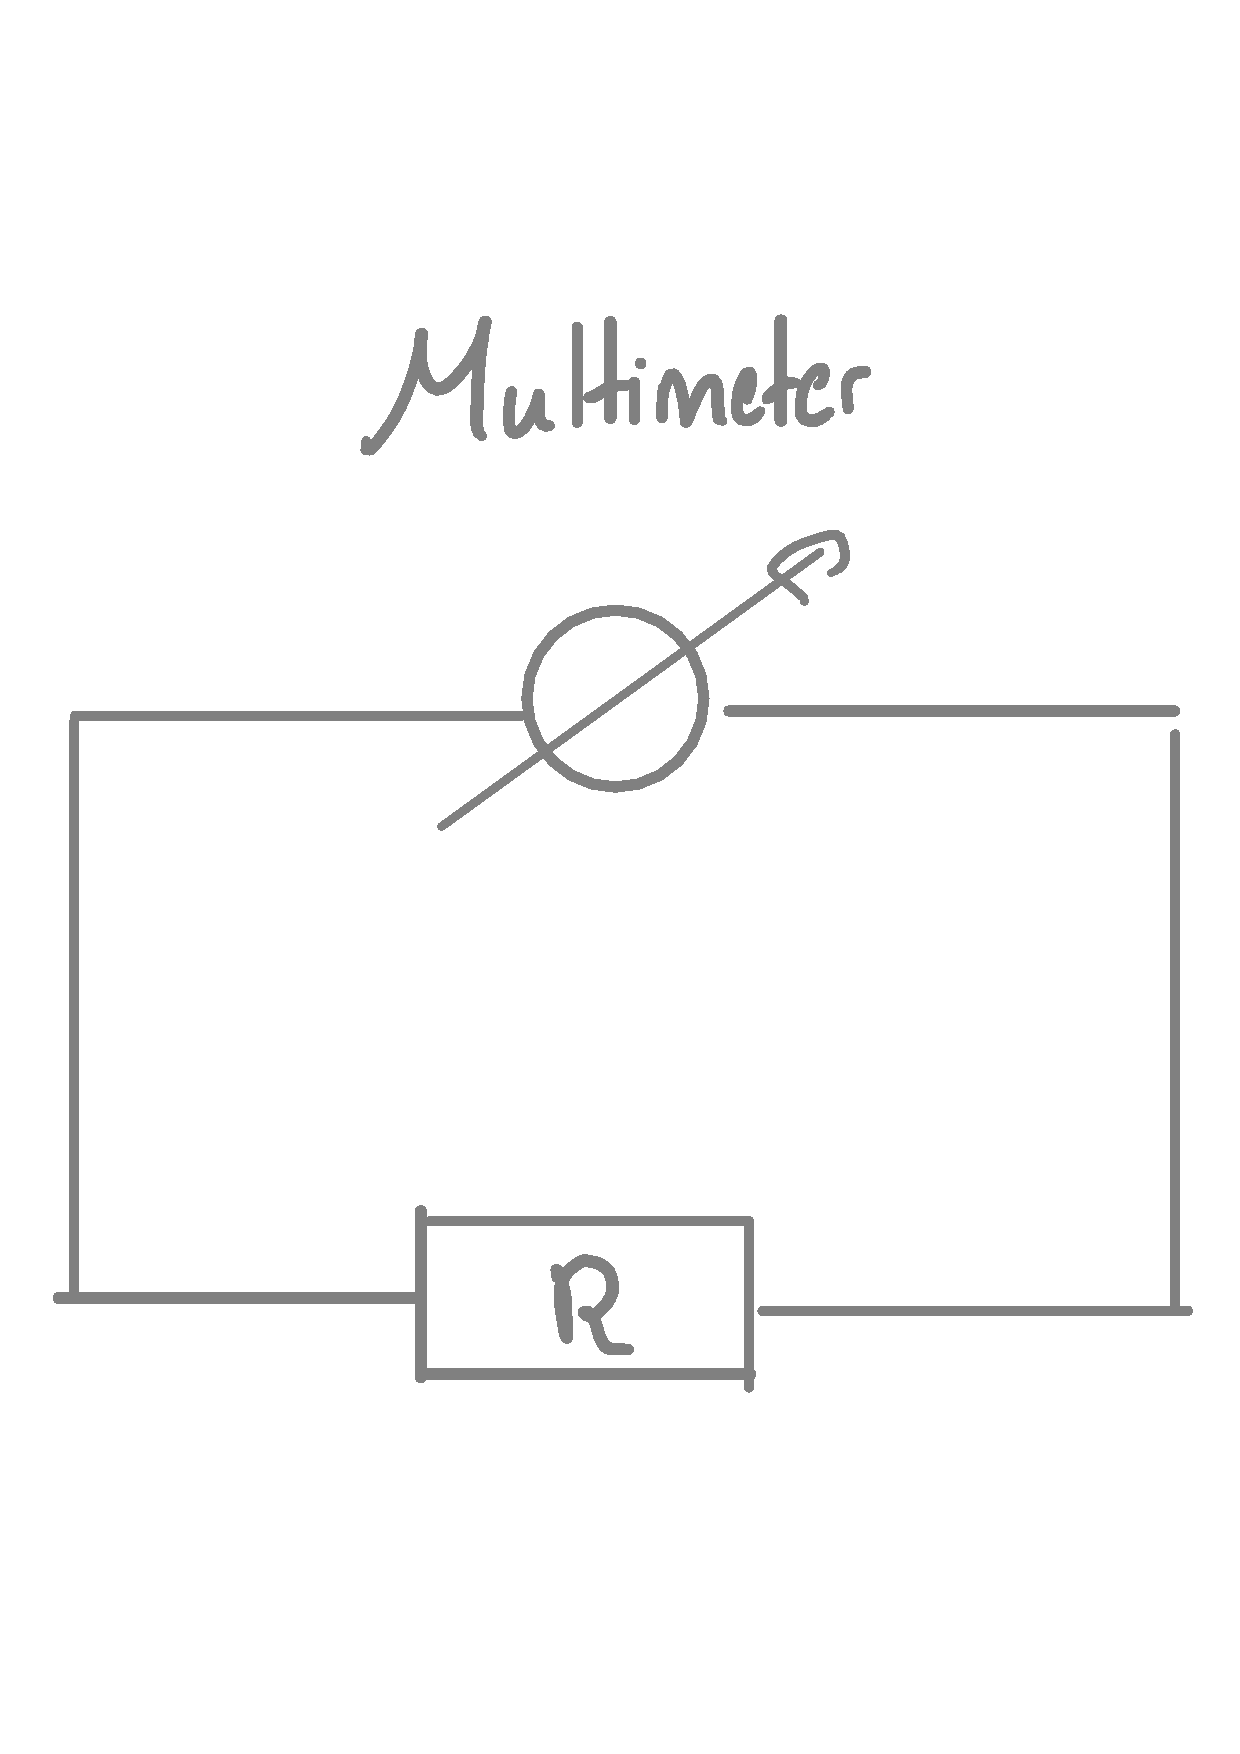
\includegraphics[width=0.5\textwidth]{Schaltung_R_Multimeter.pdf}\label{fig:f1}}
      \hfill
      \subfloat[Bilder der Schaltung]{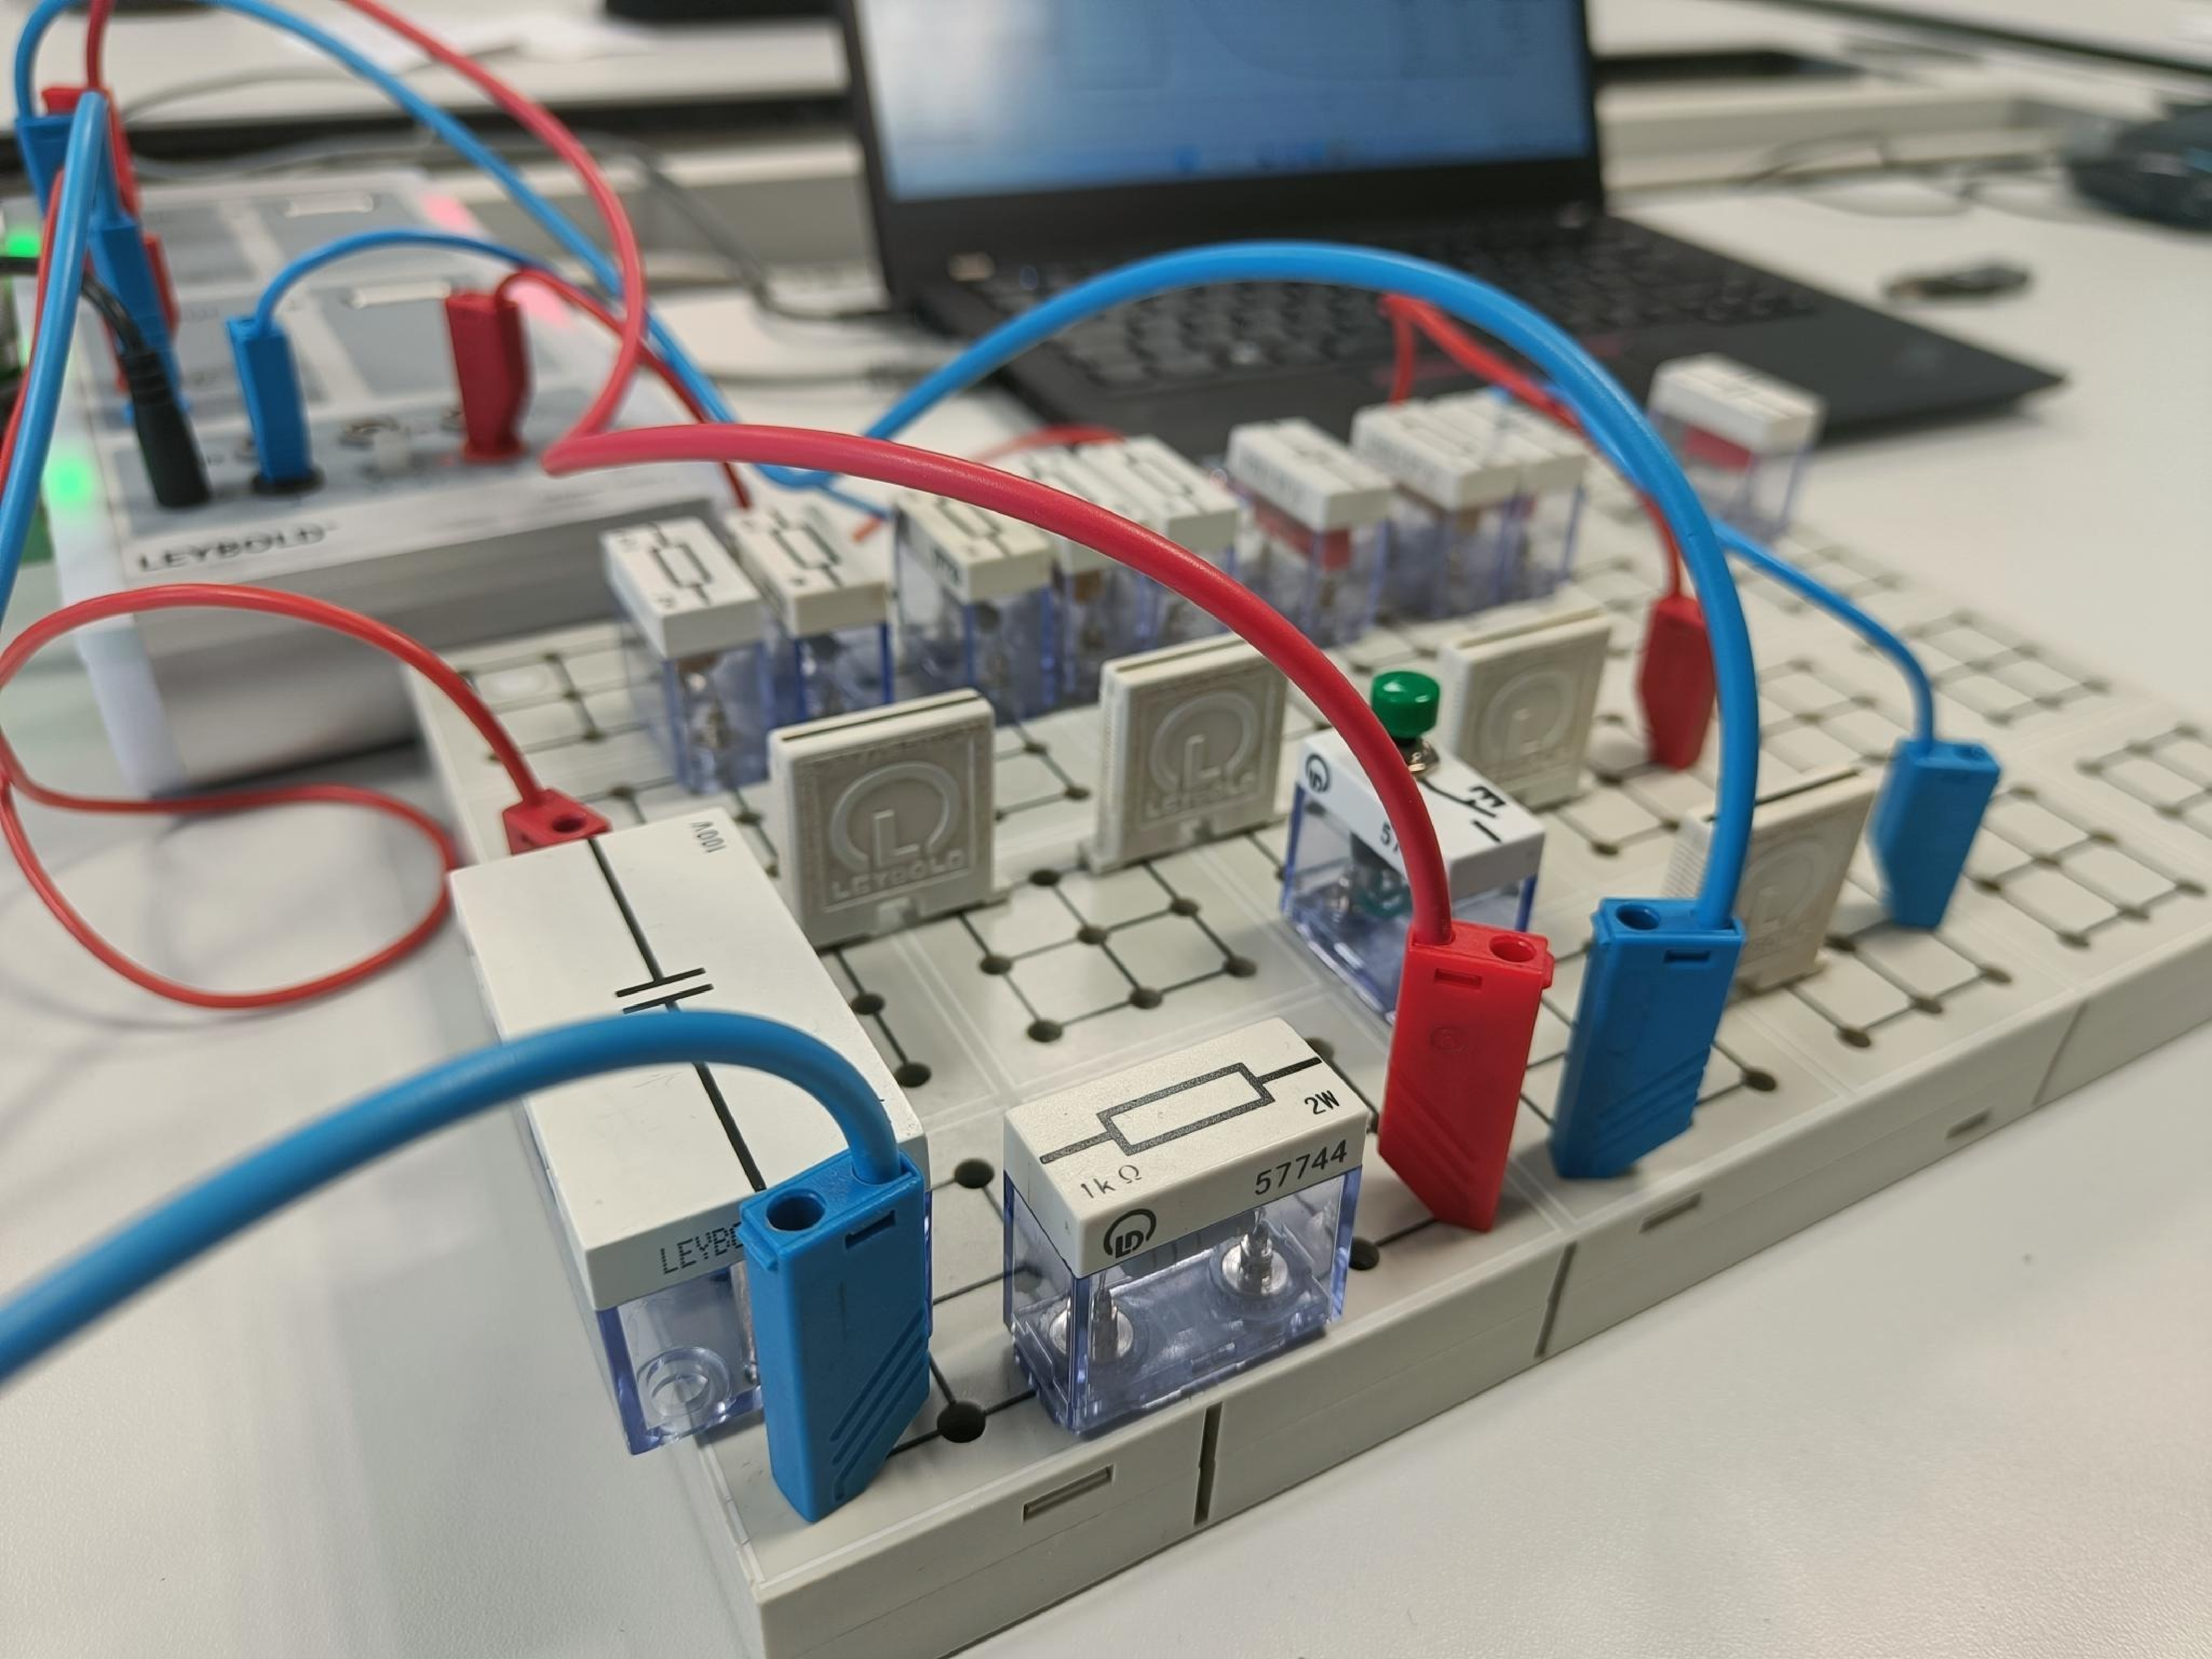
\includegraphics[width=0.5\textwidth]{Bilder_Osziloskop/Schaltung_CASSY_nah.pdf}\label{fig:f2}}
      \caption{Schaltung zur Bestimmung der Kapazität mit Cassy}
  \end{figure}
  
 Der oben stehenden Skizze und Bild können Sie den Aufbau der Schaltung entnehmen. 

\end{aufgabe}


\begin{aufgabe}{Zusammenfassung und Diskussion}
  Fassen Sie Ihre Ergebnisse zu den Kapazitäten zusammen und
  vergleichen Sie sie untereinander, mit den Messungen aus dem
  Vorversuch und mit den Herstellerangaben (Toleranz
  $\SI{5}{\percent}$).  
\end{aufgabe}
 
\end{document}

%TODO : Pythen Programm benennen, und am anfang der Auswertung rein bringen
%TODO : Bei OSZILLOSKOP Mit Wiederstand die Kapazität bestimmen aus Tau
%TODO : Korrektur von 11 Messwerten zu 10 Mesungen auf dem Protokoll
%TODO : Verwendete Formelzeichen/ eingeführte größen benennen
